% !TeX spellcheck = en_GB

%%%%%%%%%%%%%%%%%%%%%%%%%%%%%%%%%%%%%%%%%%%%%%%%%%%%%%%%%%%%%%%%%%%%%%%%%%
%%%%%%%%% Observation agreement %%%%%%%%%%%%%%
\section{Agreement between surface observations} 
%%%%%%% image scatter obs ret %%%%%%%%%%%%%%%%
\begin{figure}[t]
	\centering
    \begin{subfigure}[b]{0.38\textwidth}
    	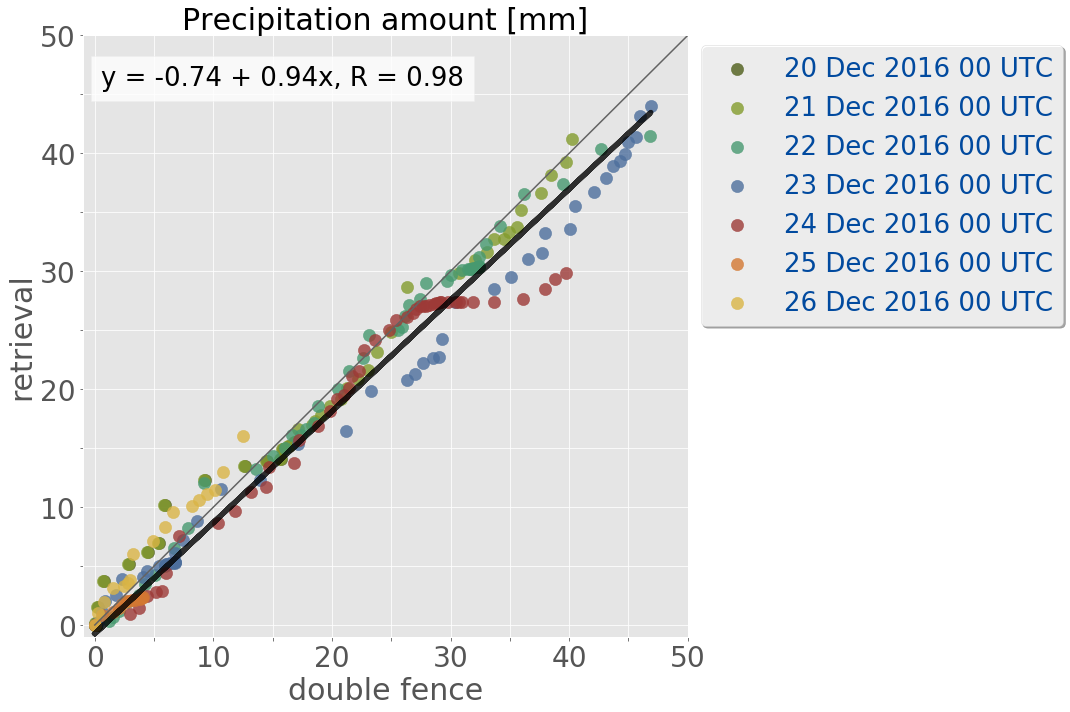
\includegraphics[trim={0.cm 0.cm 13cm 0cm},clip,
    width=\textwidth]{./fig_obs_ret/obs_ret_20161220_26_00}
    \caption{}\label{fig:res:obs_ret_scatter}
    \end{subfigure}
    %
    \begin{subfigure}[b]{0.59\textwidth}
    	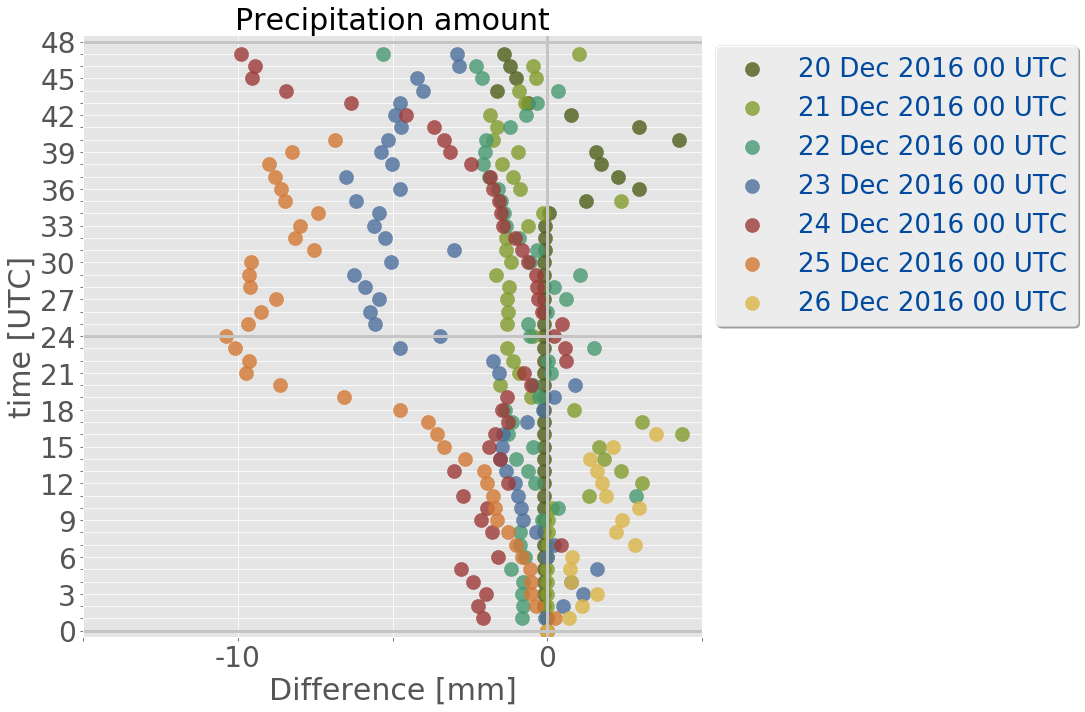
\includegraphics[trim={0.cm 0.cm 0cm 0cm},clip,
    width=\textwidth]{./fig_obs_ret/diff_20161220_26_00}
    \caption{}\label{fig:res:diff_ret_scatter}
    \end{subfigure}
    % label
%    \begin{subfigure}[t]{0.18\textwidth}
 %   	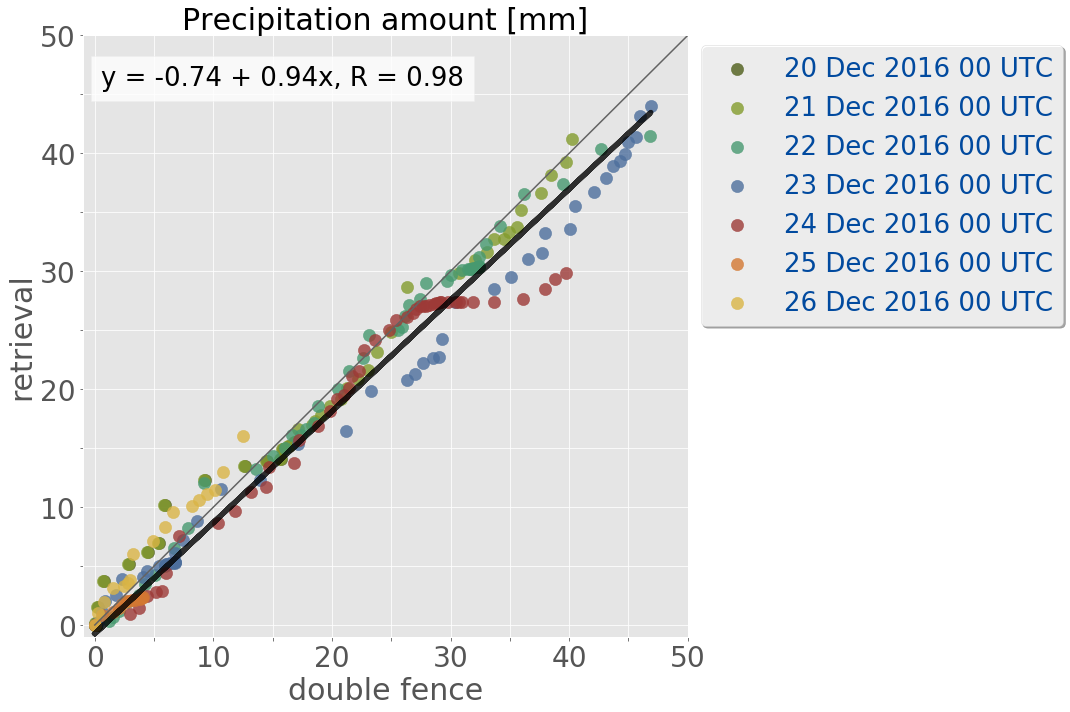
\includegraphics[trim={25.cm 13.cm 0cm 1.3cm},clip,
  %  width=\textwidth]{./fig_obs_ret/obs_ret_20161220_26_00}
   % \end{subfigure}
    
    \caption{Scatter plot comparing the observed and retrieved \SI{48}{\hour} surface accumulation (\protect\subref{fig:res:obs_ret_scatter}).  In black the linear regression between the two systems. \protect\subref{fig:res:diff_ret_scatter}: Difference between the retrieved surface accumulation and the observed accumulation by the double fence. The colours represent the days of the storm with the start of calculated \SI{48}{\hour} accumulation at \SI{0}{\UTC}. Accumulations starting on the \SI{25}{\dec} are not a fair comparison because of observed liquid precipitation. }\label{fig:res:obs_ret}
\end{figure}
%%%%%%%%%%%%%%%%%%%%%%%%%%%%%%%%%%%%%%%%%%%%%%
To be able to compare an analysis of the vertical predicted snow water content and the observed snow water content an a verification of the surface accumulation must be made. If the retrieved surface accumulation is confident in comparison to the double fence measurement then the vertical can be trusted.
\\
Comparison of the \SI{48}{\hour} accumulation demonstrate a good agreement between double fence observations and retrieved surface accumulation. \Cref{fig:res:obs_ret_scatter} shows the agreement between the two systems. The black line in \Cref{fig:res:obs_ret_scatter} presents a linear correlation with a coefficient of R = \num{0.97}. 
\\
In general underestimates the surface snowfall accumulation. \Cref{fig:res:diff_ret_scatter} shows the difference between retrieved accumulation and observed accumulation by the double fence. For \SIrange{20}{24}{\dec} \Cref{fig:res:diff_ret_scatter} indicates an underestimation of less than \SI{-5}{\mm} for the first \SI{24}{\hour}. After \SI{24}{\hour} shows especially the \SI{23}{\dec} an underestimation of up to \SI{-6.5}{\mm} and \SI{24}{\dec} underestimates larger than \SI{-6.3}{\mm} after \SI{43}{\hour}. The mean absolute error of all days is $\pm$\SI{2.06}{\mm} (excluding values on \SI{25}{\dec} after \SI{12}{\UTC} because of liquid precipitation and on \SI{26}{\dec} after \SI{17}{\UTC} because of attenuation at the MRR). The error is only representative for the Christmas storm, more storms should be investigated to find the absolute correlation between surface observation and estimated accumulation by using vertical data.
Since the bias is not large between double fence observations and retrieved surface accumulation can the vertical retrieved snow water content be trusted. 

%%%%%%%%%%%%%%%%%%%%%%%%%%%%%%%%%%%%%%%%%%%%%%%%%%%%%%%%%%%%%%%%%%%%%%%%%%

%%%%%%%%%%%%%%%%%%%%%%%%%%%%%%%%%%%%%%%%%%%%%%%%%%%%%%%%%%%%%%%%%%%%%%%%%%
%%%%%%%%% Synoptic Phenomena observed? %%%%%%%%%%%%%%
\section{Observation of large scale weather phenomena at the surface}
%%%%%%% image scatter obs ret %%%%%%%%%%%%%%%%
\begin{figure}[h!]
	\centering
    % sfc pressure
    \begin{subfigure}[b]{0.49\textwidth}
    	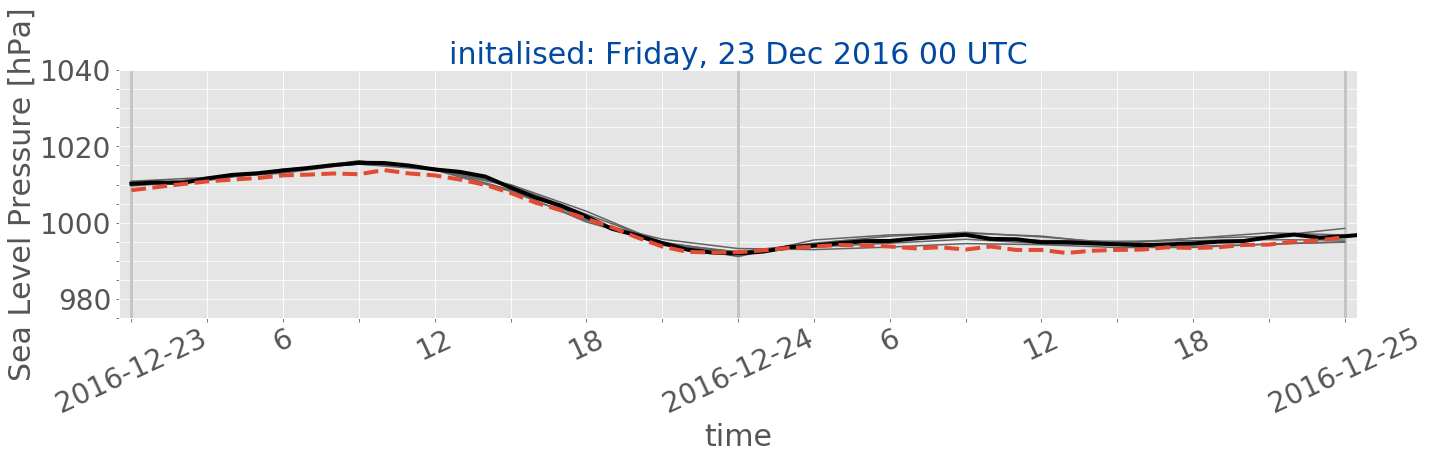
\includegraphics[trim={0.cm 3.6cm 0cm 0cm},clip,
    width=\textwidth]{./fig_sfc_pressure/20161223_00}
    	\caption{}\label{fig:res:sfc_pres23}
    \end{subfigure}
    %
    \begin{subfigure}[b]{0.49\textwidth}
    	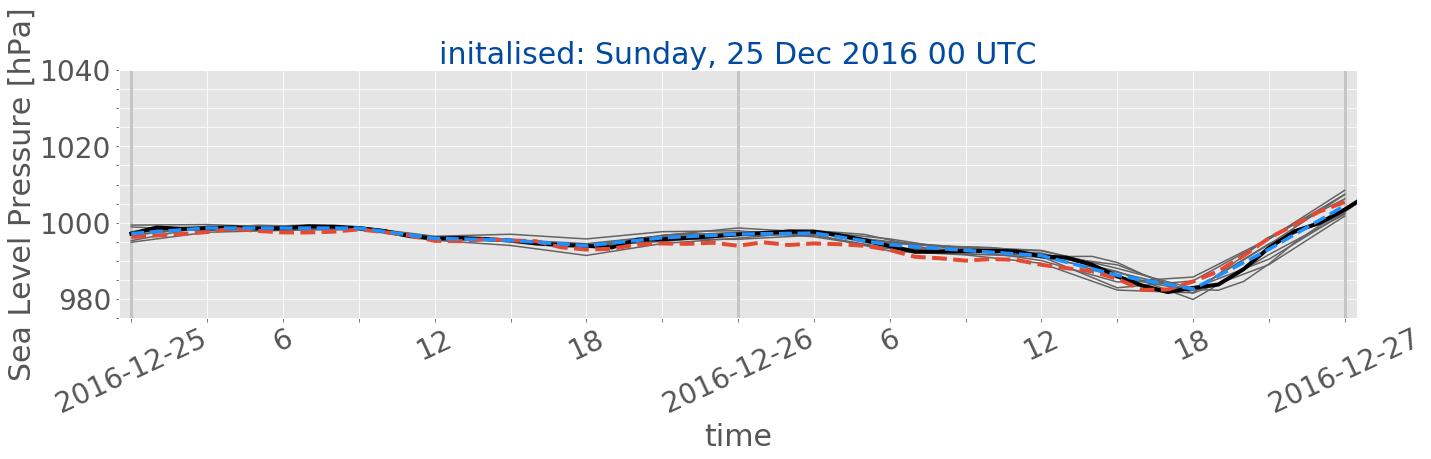
\includegraphics[trim={0.cm 3.6cm 0cm 0cm},clip,
    width=\textwidth]{./fig_sfc_pressure/20161225_00}
    	\caption{}\label{fig:res:sfc_pres25}
    \end{subfigure}
    % sfc temp
    \begin{subfigure}[b]{0.49\textwidth}
    	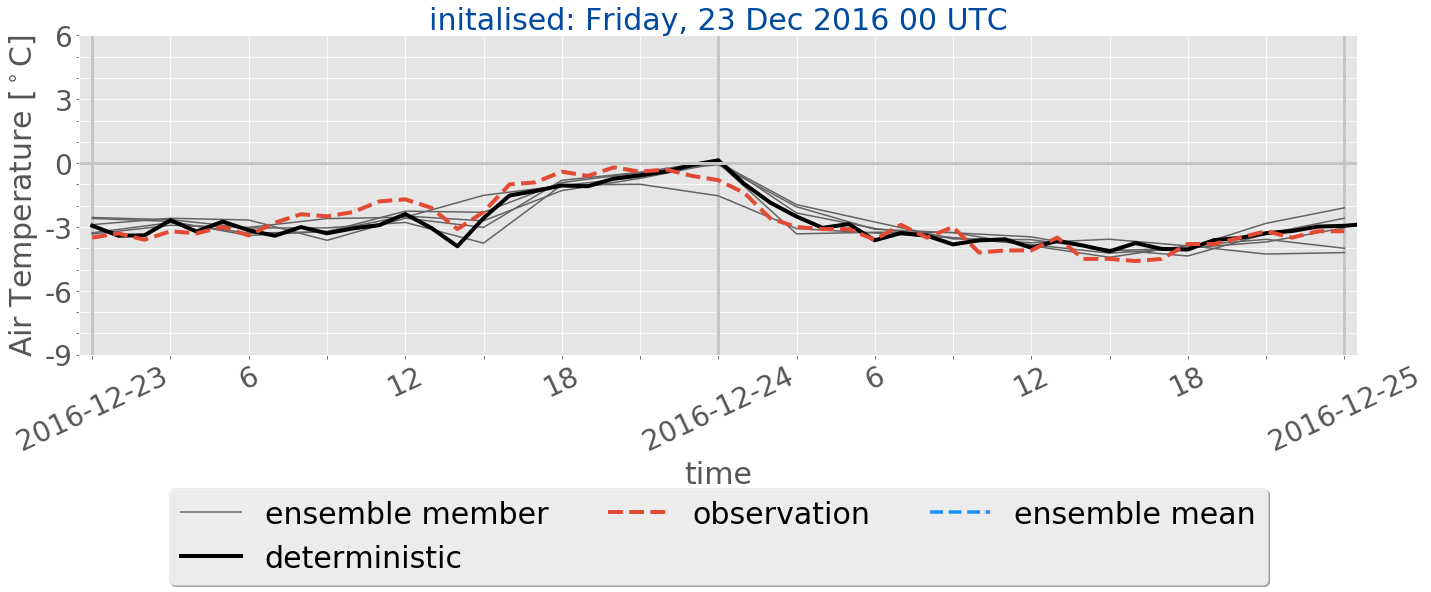
\includegraphics[trim={0.cm 3.6cm 0cm 0cm},clip,
    width=\textwidth]{./fig_sfc_temp/20161223_00}
    	\caption{}\label{fig:res:sfc_temp23}
    \end{subfigure}
    %
    \begin{subfigure}[b]{0.49\textwidth}
    	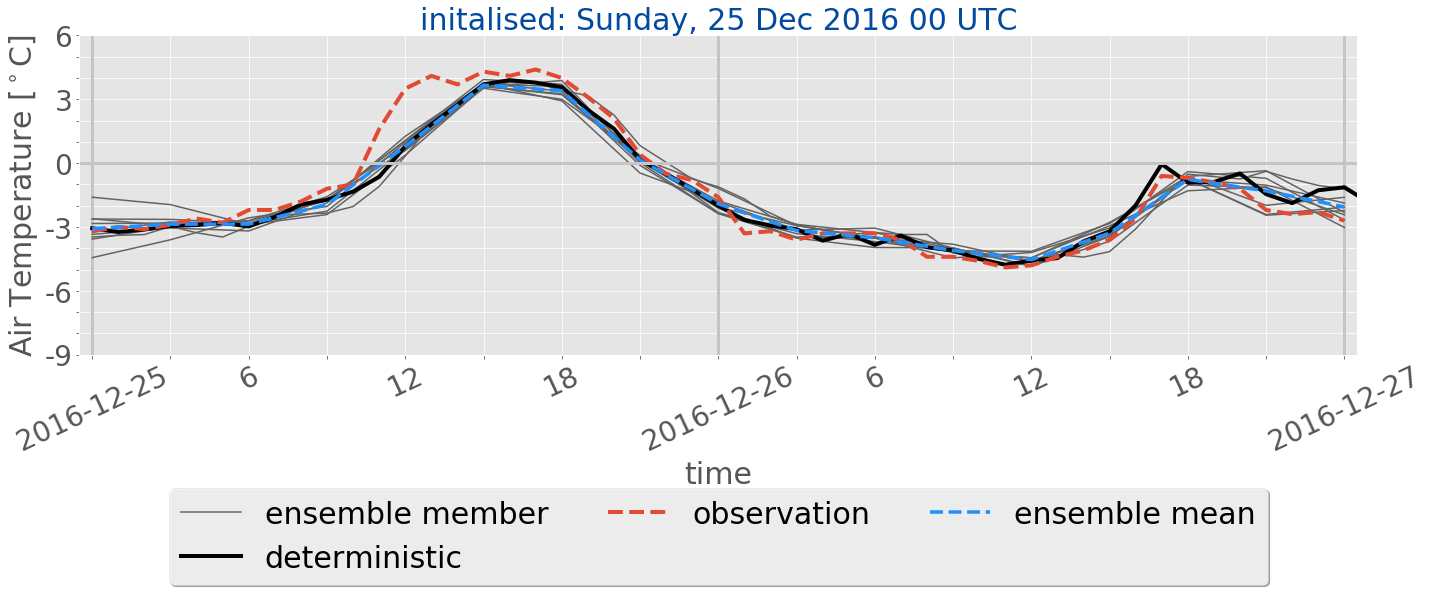
\includegraphics[trim={0.cm 3.6cm 0cm 0cm},clip,
    width=\textwidth]{./fig_sfc_temp/20161225_00}
    	\caption{}\label{fig:res:sfc_temp25}
    \end{subfigure}
    % sfc wd
    \begin{subfigure}[b]{0.49\textwidth}
    	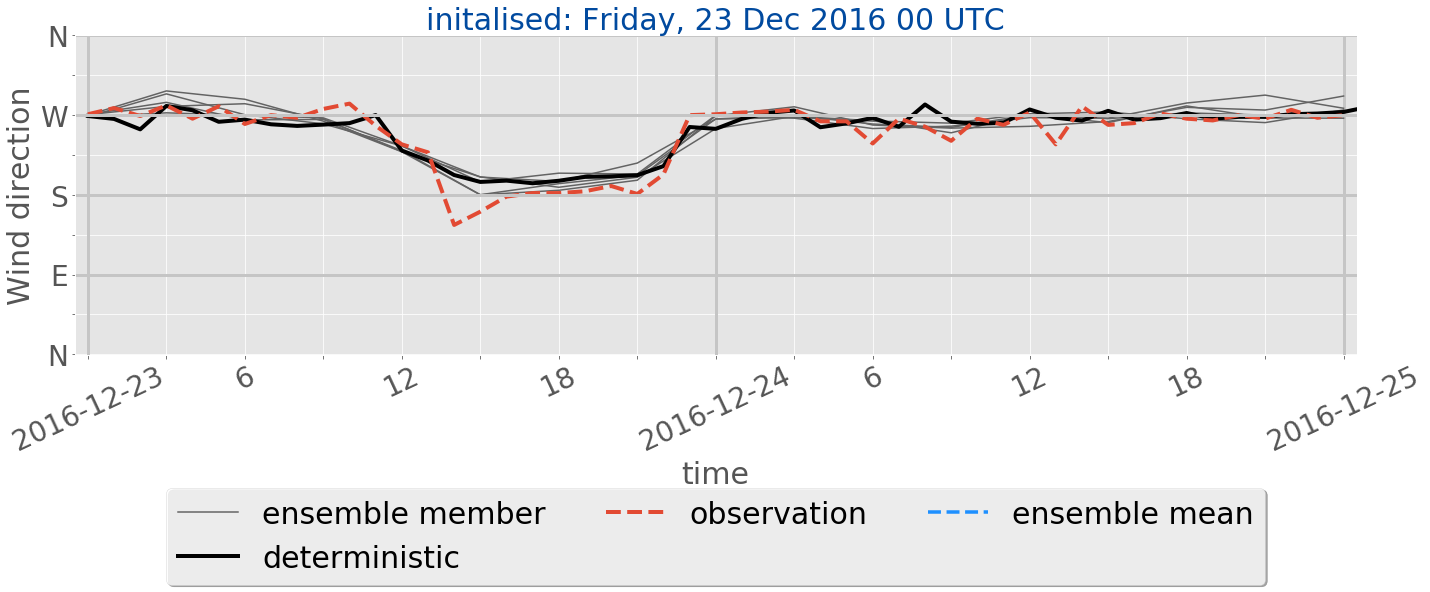
\includegraphics[trim={0.cm 3.6cm 0cm 0cm},clip,
    width=\textwidth]{./fig_sfc_wd/20161223_00}
    	\caption{}\label{fig:res:sfc_wd23}
    \end{subfigure}
    %
    \begin{subfigure}[b]{0.49\textwidth}
    	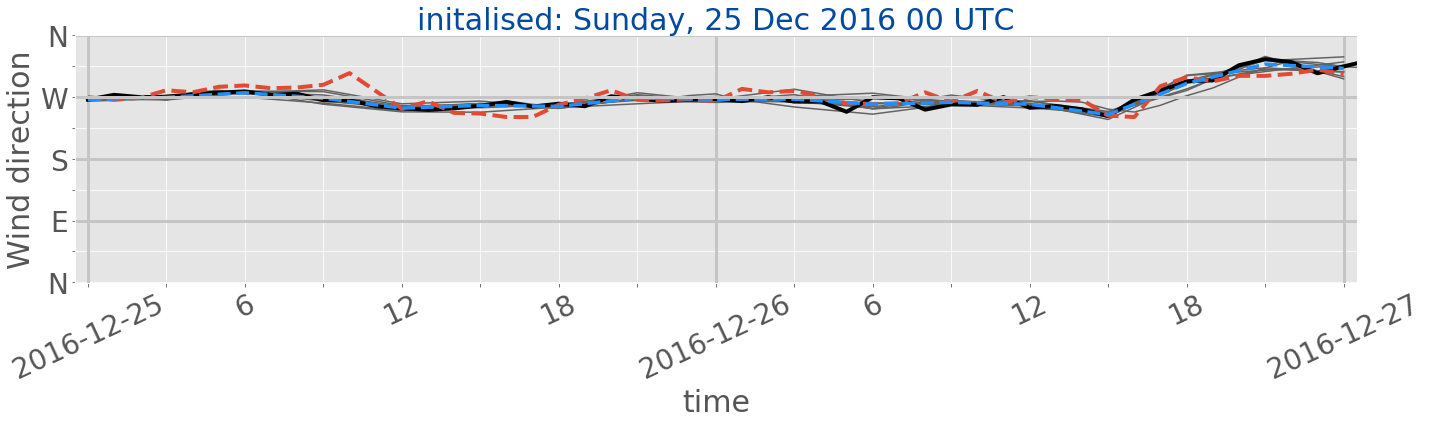
\includegraphics[trim={0.cm 3.6cm 0cm 0cm},clip,
    width=\textwidth]{./fig_sfc_wd/20161225_00}
    	\caption{}\label{fig:res:sfc_wd25}
    \end{subfigure}
    % sfc ws
    \begin{subfigure}[b]{0.49\textwidth}
    	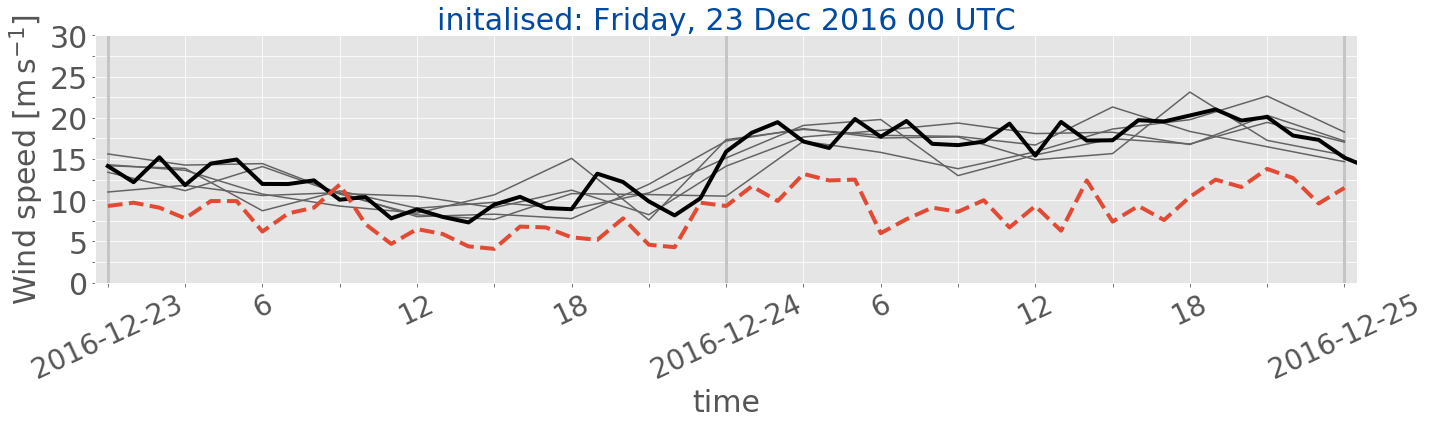
\includegraphics[trim={0.cm 3.6cm 0cm 0cm},clip,
    width=\textwidth]{./fig_sfc_ws/20161223_00}
    	\caption{}\label{fig:res:sfc_ws23}
    \end{subfigure}
    %
    \begin{subfigure}[b]{0.49\textwidth}
    	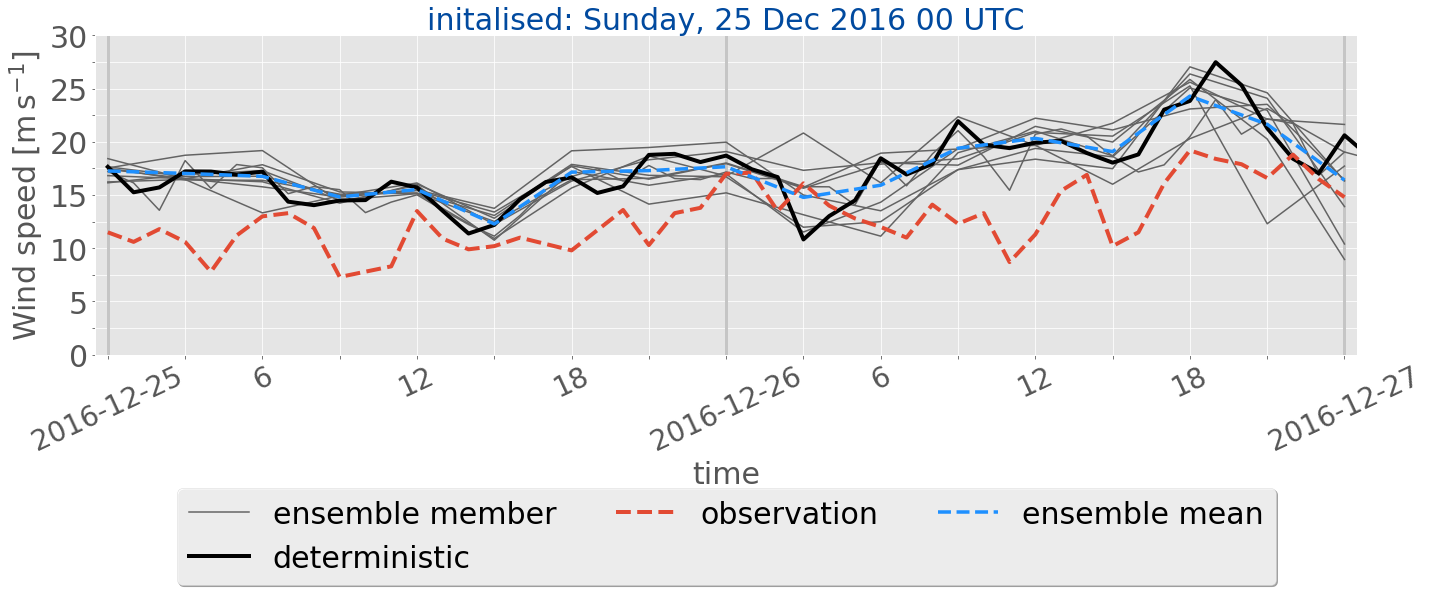
\includegraphics[trim={0.cm 3.6cm 0cm 0cm},clip,
    width=\textwidth]{./fig_sfc_ws/20161225_00}
    	\caption{}\label{fig:res:sfc_ws25}
    \end{subfigure}
    % sfc precip
    \begin{subfigure}[b]{0.49\textwidth}
    	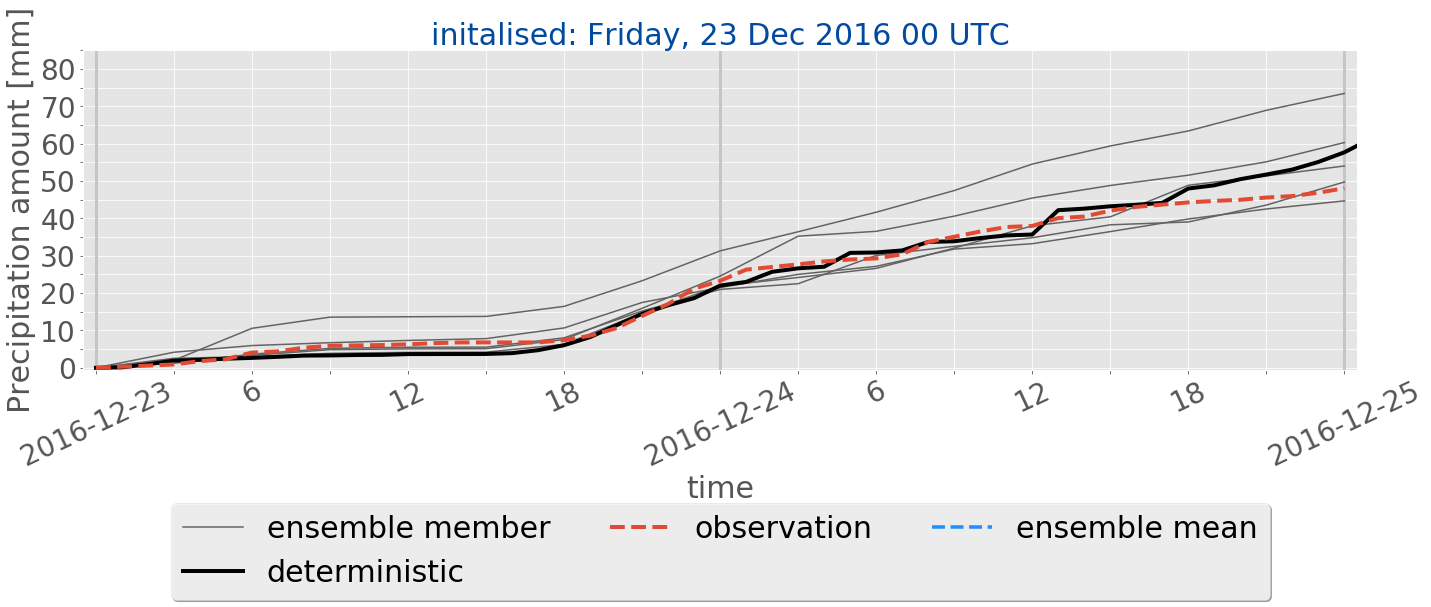
\includegraphics[trim={0.cm 3.6cm 0cm 0cm},clip,
    width=\textwidth]{./fig_sfc_precip/20161223_00}
    	\caption{}\label{fig:res:sfc_precip23}
    \end{subfigure}
    %
    \begin{subfigure}[b]{0.49\textwidth}
    	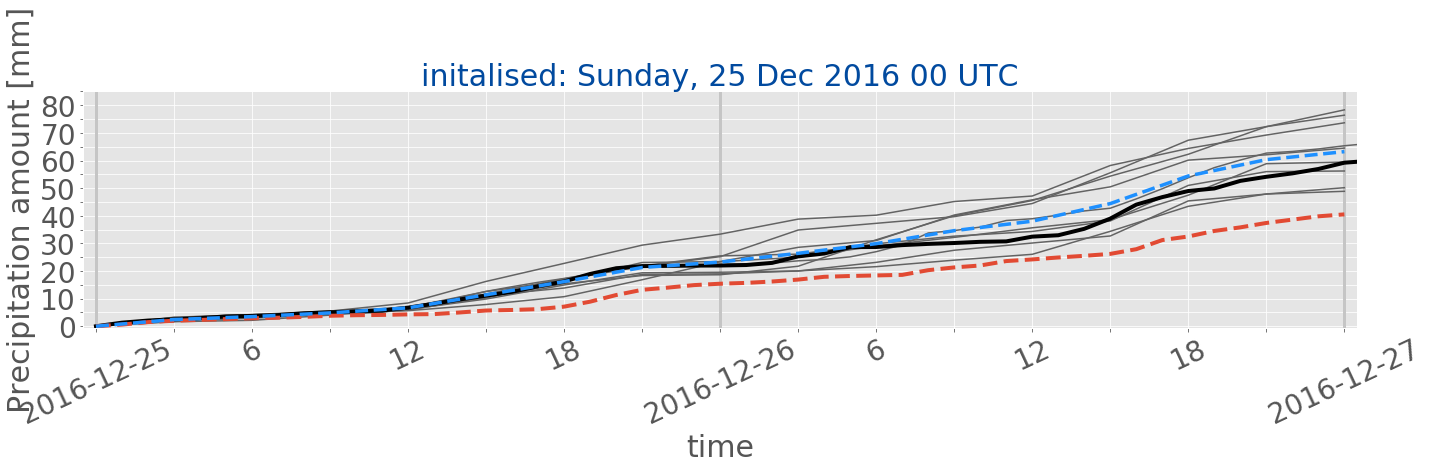
\includegraphics[trim={0.cm 3.6cm 0cm 0cm},clip,
    width=\textwidth]{./fig_sfc_precip/20161225_00}
    	\caption{}\label{fig:res:sfc_precip25}
    \end{subfigure}
    
    % label
    \begin{subfigure}[b]{\textwidth}
    \centering
 		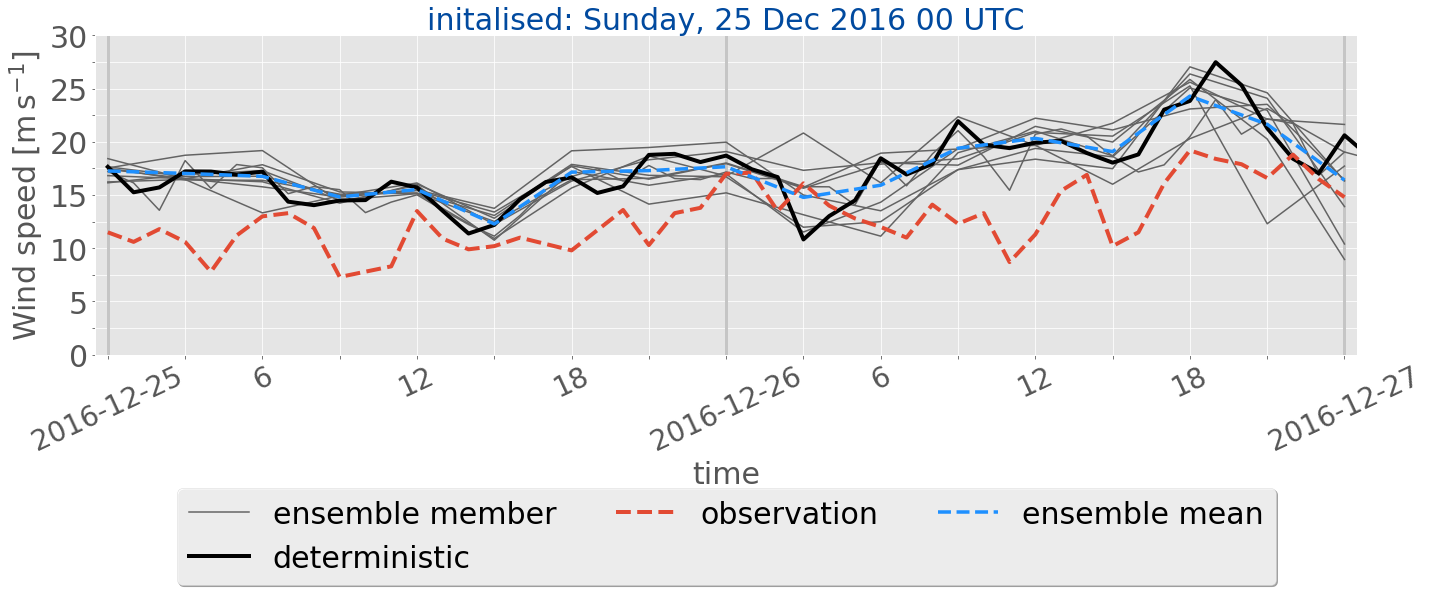
\includegraphics[trim={5.5cm 0cm 5.cm 17.2cm},clip,
    width=0.6\textwidth]{./fig_sfc_ws/20161225_00}
    \end{subfigure}
    %
\end{figure}
\begin{figure}\ContinuedFloat
	\centering
    % sfc pressure
    \begin{subfigure}[b]{0.49\textwidth}
		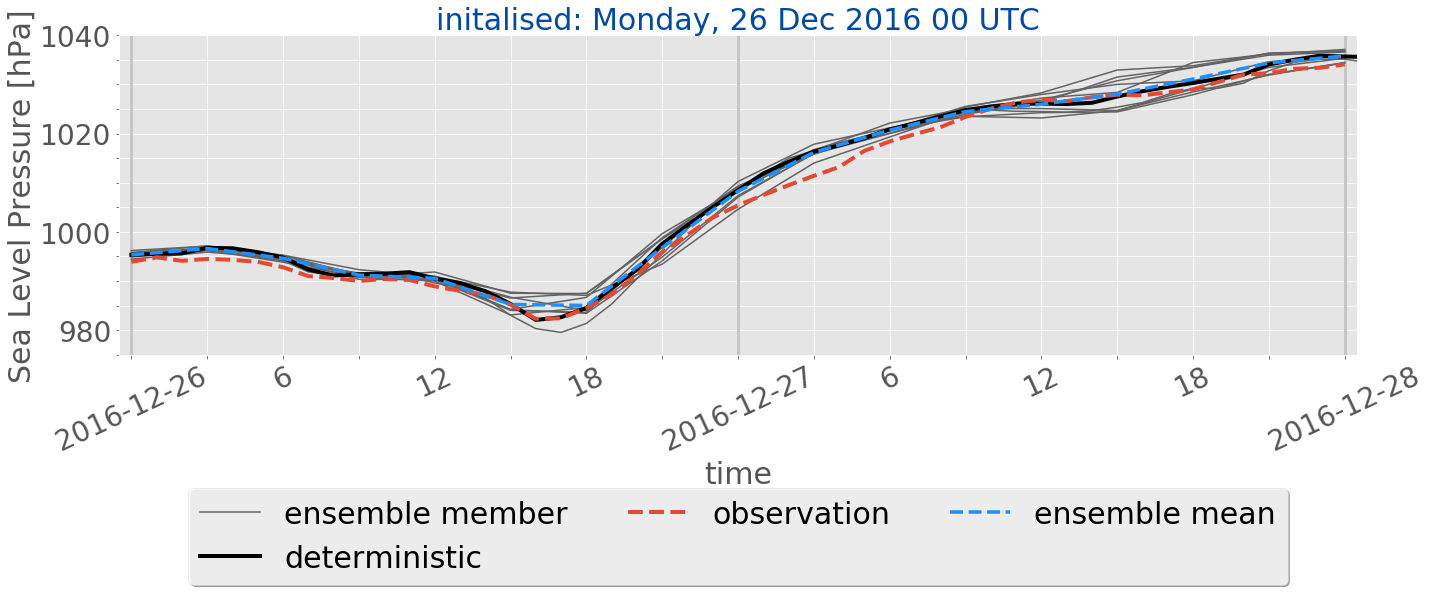
\includegraphics[trim={0.cm 3.6cm 0cm 0cm},clip,
    width=\textwidth]{./fig_sfc_pressure/20161226_00}
    	\caption{}\label{fig:res:sfc_pres26}
	\end{subfigure}
    
    % sfc temp
    \begin{subfigure}[b]{0.49\textwidth}
    	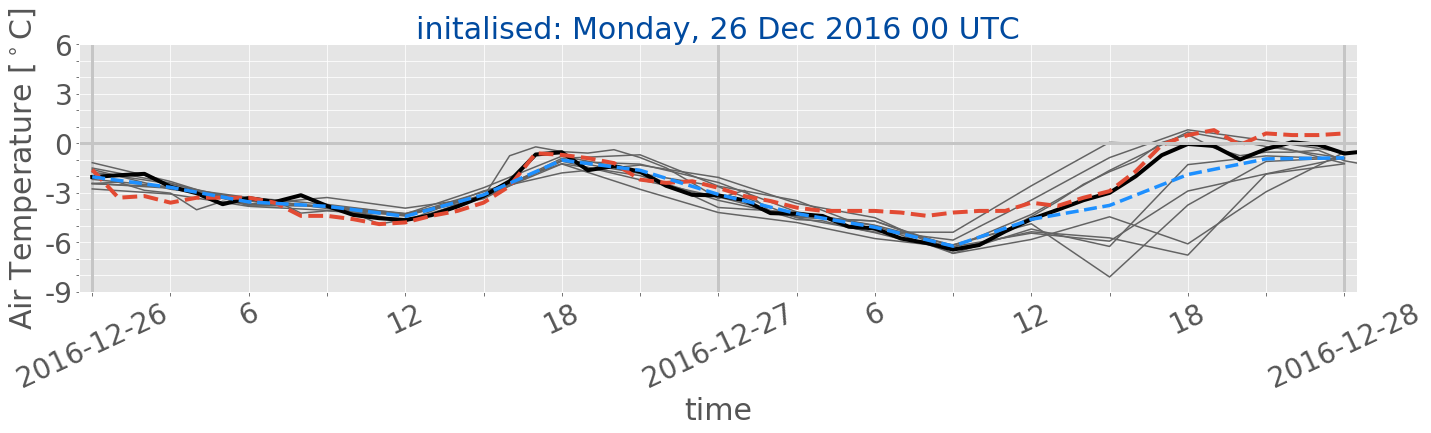
\includegraphics[trim={0.cm 3.6cm 0cm 0cm},clip,
    width=\textwidth]{./fig_sfc_temp/20161226_00}
    	\caption{}\label{fig:res:sfc_temp26}
    \end{subfigure}
    
    % sfc wd
    \begin{subfigure}[b]{0.49\textwidth}
    	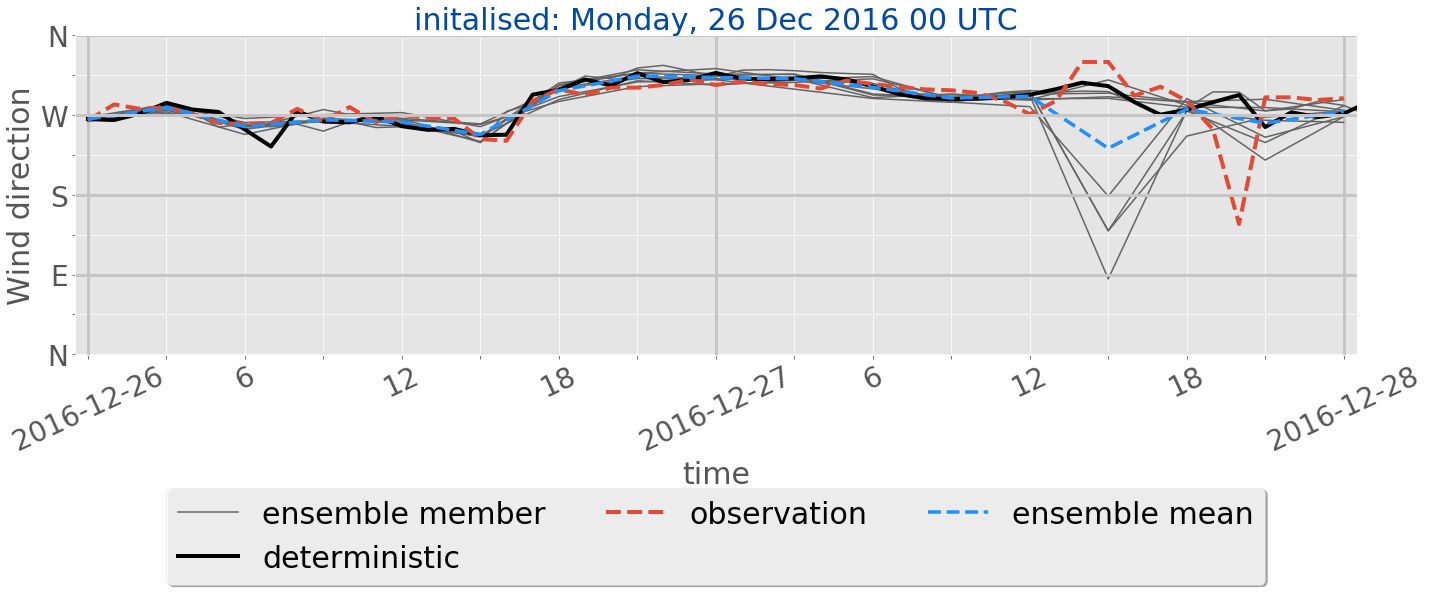
\includegraphics[trim={0.cm 3.6cm 0cm 0cm},clip,
    width=\textwidth]{./fig_sfc_wd/20161226_00}
    	\caption{}\label{fig:res:sfc_wd26}
    \end{subfigure}
    
    % sfc ws
    \begin{subfigure}[b]{0.49\textwidth}
    	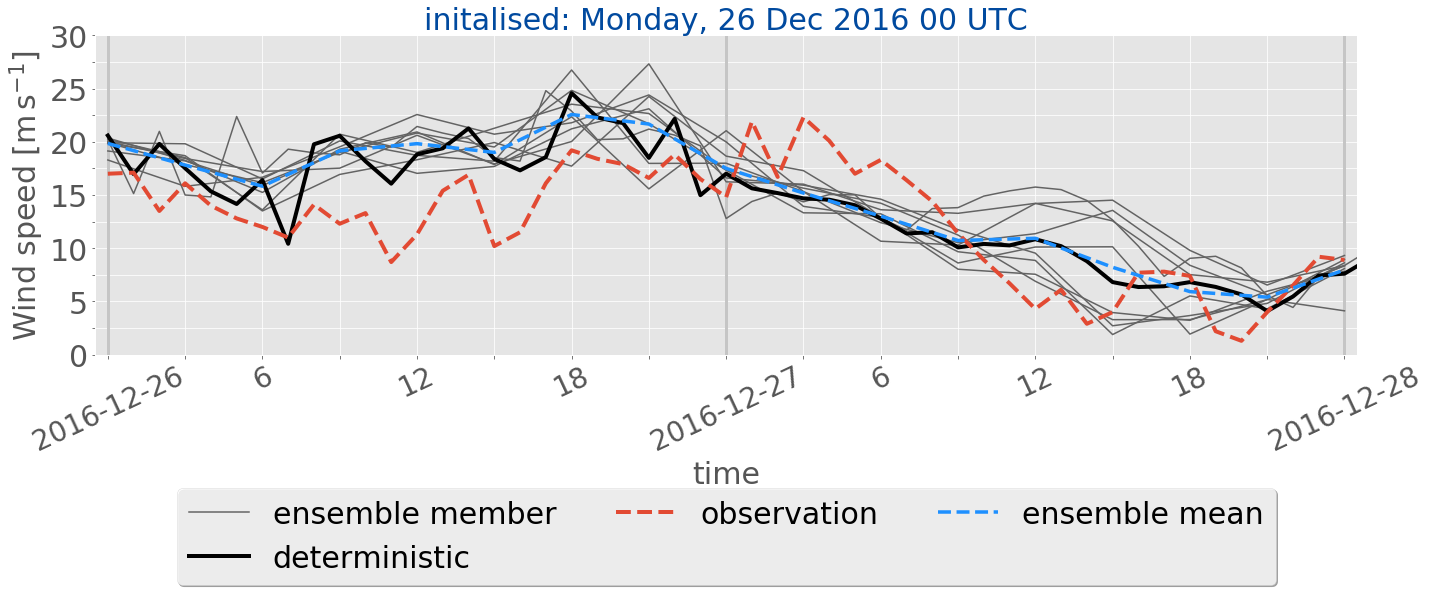
\includegraphics[trim={0.cm 3.6cm 0cm 0cm},clip,
    width=\textwidth]{./fig_sfc_ws/20161226_00}
    	\caption{}\label{fig:res:sfc_ws26}
    \end{subfigure}
    
    % sfc precip
    \begin{subfigure}[b]{0.49\textwidth}
    	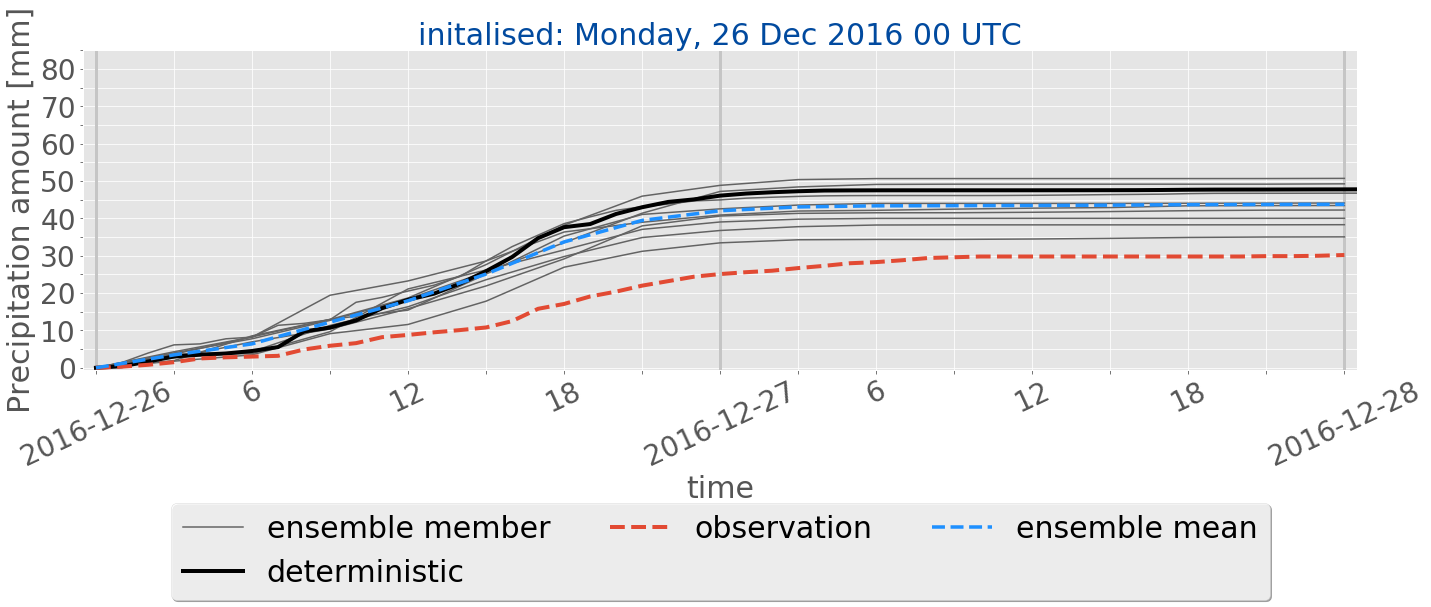
\includegraphics[trim={0.cm 3.6cm 0cm 0cm},clip,
    width=\textwidth]{./fig_sfc_precip/20161226_00}
    	\caption{}\label{fig:res:sfc_precip26}
    \end{subfigure}
    
    % label
    \begin{subfigure}[b]{\textwidth}
    	\centering
 		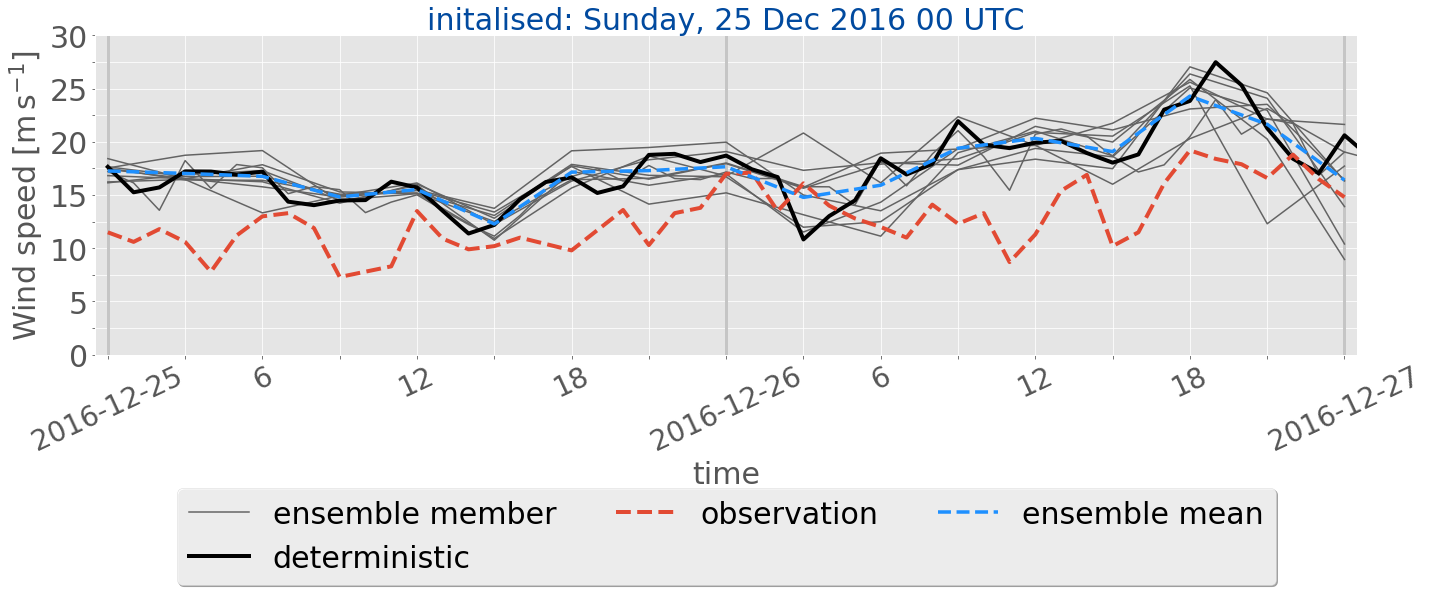
\includegraphics[trim={5.5cm 0cm 5.cm 17.2cm},clip,
    width=0.6\textwidth]{./fig_sfc_ws/20161225_00}
    \end{subfigure}
    \caption{\SI{48}{\hour} surface observations and ensemble forecasts initialised on the \SI{23}{\dec} (left column, previous page, \protect\subref{fig:res:sfc_pres23}, \protect\subref{fig:res:sfc_temp23}, \protect\subref{fig:res:sfc_wd23}, \protect\subref{fig:res:sfc_ws23}, \protect\subref{fig:res:sfc_precip23}), and on \SI{25}{\dec} (right column, previous page, \protect\subref{fig:res:sfc_pres25}, \protect\subref{fig:res:sfc_temp25}, \protect\subref{fig:res:sfc_wd25}, \protect\subref{fig:res:sfc_ws25}, \protect\subref{fig:res:sfc_precip25}) as well as \SI{25}{\dec} (\protect\subref{fig:res:sfc_pres26}, \protect\subref{fig:res:sfc_temp26}, \protect\subref{fig:res:sfc_wd26}, \protect\subref{fig:res:sfc_ws26}, \protect\subref{fig:res:sfc_precip26}). Line representation according to the label. Upper panel sea level pressure, second \SI{2}{\metre} air temperature, third and forth \SI{10}{\metre} wind direction and speed, respectively, and lowest panel precipitation amount. }\label{fig:res:sfc_obs_meps}
\end{figure}
%%%%%%%%%%%%%%%%%%%%%%%%%%%%%%%%%%%%%%%%%%%%%%
One of the main factors, that made this particular case so interesting is the fact, that several times in the six day period frontal boundaries passed over Norway. The aim of this work is to determine if large scale features were observed at the measurement site. 
\\
When comparing the MEPS forecast of surface weather maps and the ECMWF analysis of dynamic tropopause maps, it shows that frontal passages occurred on three days during the Christmas storm (\Cref{fig:GeopJet} and \ref{fig:DynTropo}).  These frontal boundaries show in the surface observations and ensemble forecasts on \SIlist{23;25;26}{\dec}. A typical cyclone has a prevailing warm front and a faster moving cold front. As the storm gets more intense and the cold front rotates around the low pressure centre and catches the warm front. This follows an occluded front. Changes in pressures, temperature, wind direction and wind speed can occur. In some cases an intensification of the precipitation can be observed as well.
\\
\Cref{fig:res:sfc_obs_meps} shows the different parameters forecasts initialised at \SI{00}{\UTC} for \SIlist{23;25;26}{\dec}, as well as the observations at the Haukeliseter measurement site in dash-red.
Typical pressure decreases and increases, as well as temperature increases and wind changes are present on \SIlist{23;26}{\dec}. The \SI{25}{\dec} shows only a passage of a warm air mass. 
\\
As described in \Cref{sec:largeScale} shows the ECMWF dynamic tropopause analysis map (\Cref{fig:DT23}) more ridging and therefore warmer air over Southern Norway on \SI{23}{\dec}. The low pressure system approaches in the course of the day south-east Iceland and hence stronger west to south west wind are associated with the cyclone (\Cref{fig:GP23}). The MEPS forecast, initialised on \SI{23}{\dec} \SI{0}{\UTC} in \Cref{fig:res:sfc_pres23} shows the decrease in pressure after \SI{12}{\UTC} due to the passage of the occluded front with a constant pressure after the transition. Since warmer air is more advected to the North and the DT in \Cref{fig:DT23} shows a warmer low pressure core, an increase in temperature was observed and predicted at the measurement site (\Cref{fig:res:sfc_temp23}). 
\\
As the cyclone is advected to the north-east, closer into the Norwegian Sea, a wind change can be seen in the analysis map from ECMWF (\Cref{fig:GP23}, were first west wind and later south-west wind was associated with the low pressure system. In \Cref{fig:res:sfc_wd23} and \subref{fig:res:sfc_ws23} a similar wind change can be observed by the MEPS forecast and observations.
\\
On \SI{23}{\dec} was the passage of the occlusion also observed by an increase in precipitation. Before \SI{18}{\UTC} shows the surface accumulation light precipitation. During the passage of the occluded front increases the observed surface accumulation and is associated to continuous, heavy precipitation.
\\
\\
Similar patterns were seen for the passage of the occluded front on \SI{26}{\dec} in the ECMWF analysis \Cref{fig:DT26} and \ref{fig:GP26}. In this case the low pressure system was located north of Morø og Romsdal in the Norwegian Sea. In the morning was the low cyclone located east of Iceland and in the course of the day it got closer to the coast of Norway. Before landfall at \SI{16}{\UTC} demonstrates \Cref{fig:res:sfc_pres26} a pressure decrease. During the passage the sea level pressure decreases its lowest point of \SI{985}{\hPa}, and increased afterwards during the dissipation of the Christmas storm.
\\
Since the cyclone was surrounded by colder air (south of the low pressure system) first a drop and then an increase of temperature were observed and forecasted by MEPS. An indication of the passage is also seen in the \SI{10}{\metre} wind observations and forecasts. As the cyclone is east of Iceland with a westward large scale surface wind (\Cref{fig:GP26_00} and \Cref{fig:GP26_12}), shows \Cref{fig:res:sfc_wd26} west wind wind with observed strength up to \SI{17.5}{\mPs} (\Cref{fig:res:sfc_ws26}). During the passage changes the wind direction to north-west with higher wind speed which can be associated to the location of the low pressure system and the closer surface isobars (\Cref{fig:DT26}). 
\\
The precipitation was continues throughout the day, with light to moderate precipitation before the passage and heavy precipitation around \SI{16}{\UTC} followed by moderate to light.
\\
\\
While on \SIlist{23;25}{\dec} the precipiation was associated with a passage/landfall of an occluded front, was the \SI{25}{\dec} marked by the transition of a warm sector. The ECMWF analysis showed a ridging at the DT surface. The surface cyclone core is south east of Iceland in \Cref{fig:DT25} with two associated frontal boundaries. While the warm front is aproaching the west coast, is the cold front north west of Great Britain. The cold fronts tail moved into lower latitudes, following the slow down of the cold front, leading to a stationary frontal boundary. Further more the mid-latidual jet is aligned along the surface frontal boundaries (\Cref{fig:DT25_00}), while the Haukeliseter site is located below the left jet exit region. This leads to rising motion at the surface.
\\
Neither pressure nor wind observations and forecasts indicate the passage of any frontal boundary. The only indication of the transition is seen in the increase of temperature at \SI{11}{\UTC} until \SI{21}{\UTC} (\Cref{fig:res:sfc_temp25}). In \Cref{fig:res:sfc_wd25} a small wind change was observed from west to north-west by the wind mast at \SI{10}{\UTC}, but the forecast does not show this wind change for an initialisation on \SI{25}{\dec}. 
\\
%%%%%%% image liquid obs particle %%%%%%%%%%%%%%%%
\begin{figure}[t]
	\centering
	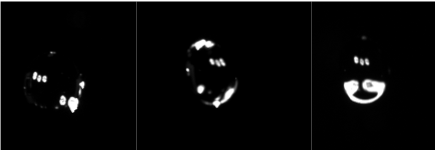
\includegraphics[%trim={45.cm 30.cm 13cm 35cm},clip,
    width=0.8\textwidth]{./MASC_obs/Masc_obs_liquid_2512}
    \caption{MASC images of falling water drops observed on \SI{25}{\dec} at \SI{17}{\UTC} from three different angles. Not all parts of the liquid sphere are equally illuminated.}\label{fig:res:obs_masc}
\end{figure}
%%%%%%%%%%%%%%%%%%%%%%%%%%%%%%%%%%%%%%%%%%%%%%
In \Cref{fig:res:obs_masc} are the surface observations from the MASC during the passage of the warm sector. Without the images taken at \SI{17}{\UTC} at the Haukeliseter site it would not be possible to verify that liquid precipitation occurred. Together with the increase in surface temperature in \Cref{fig:res:sfc_temp25} it is qualified that at least the warm sector of the low pressure system appeared at the measurement site.
\\
%%%%%%% image scatter obs ret %%%%%%%%%%%%%%%%
\begin{figure}[h!]
	\centering
    % sfc pressure
    \begin{subfigure}[b]{0.49\textwidth}
    	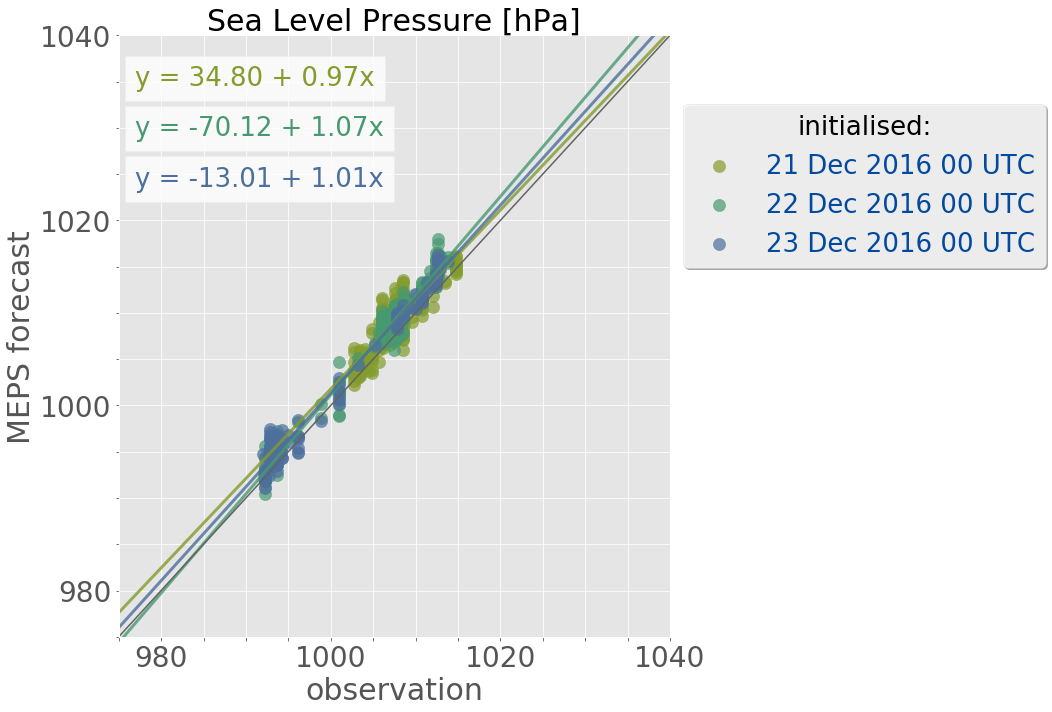
\includegraphics[trim={0.cm 0cm 12.5cm 0cm},clip,
    width=\textwidth]{./fig_sfc_pressure/obs_model_20161221_23_00}
    	\caption{}\label{fig:scat:pres2123}
    \end{subfigure}
    %
    \begin{subfigure}[b]{0.49\textwidth}
    	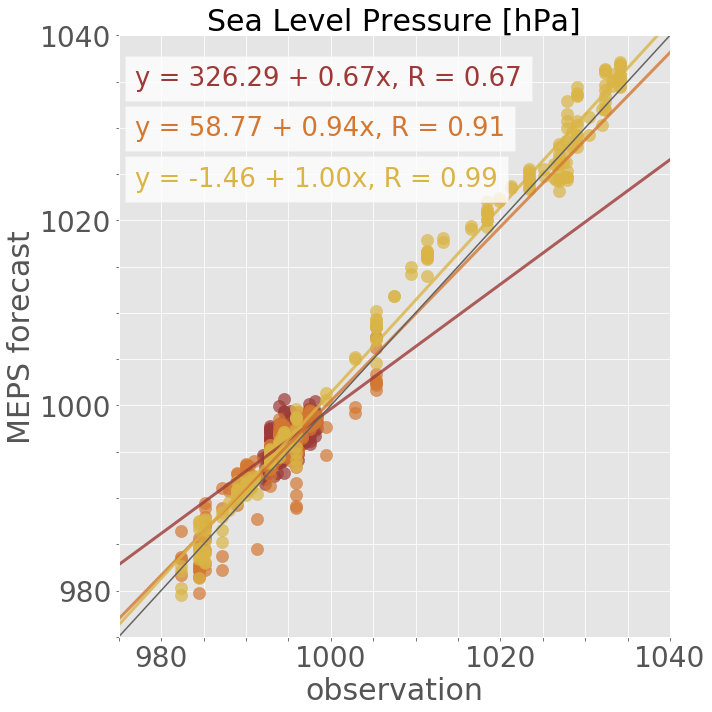
\includegraphics[trim={0.cm 0cm 12.5cm 0cm},clip,
    width=\textwidth]{./fig_sfc_pressure/obs_model_20161224_26_00}
    	\caption{}\label{fig:scat:pres2426}
    \end{subfigure}
%     % sfc temp
     \begin{subfigure}[b]{0.49\textwidth}
     	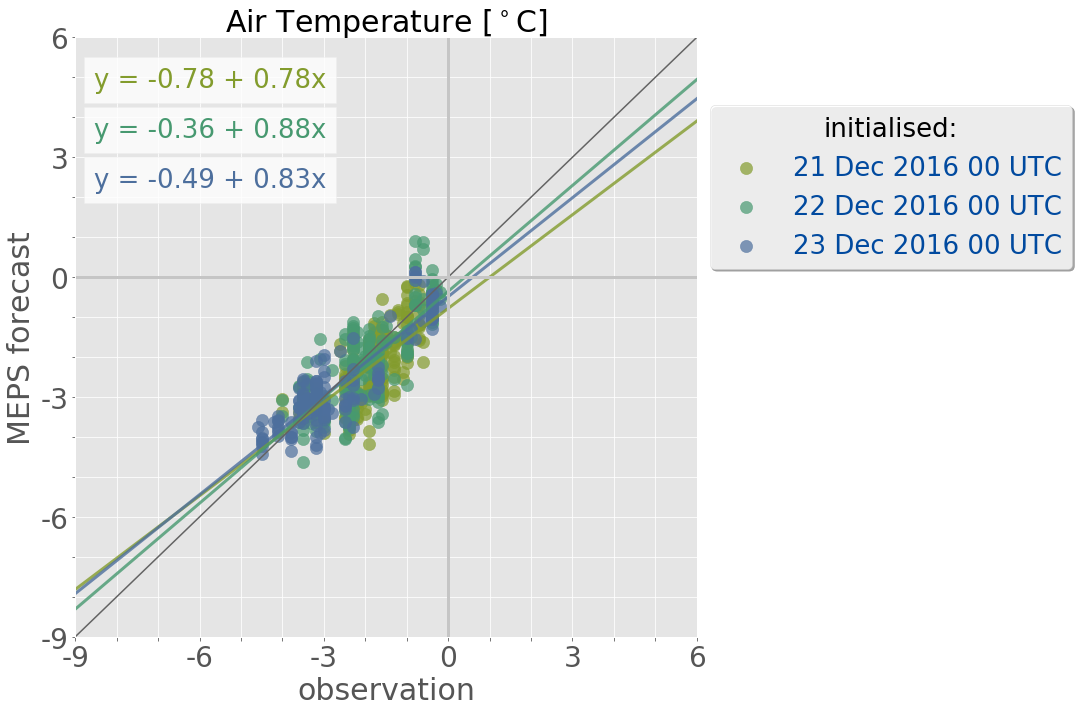
\includegraphics[trim={0.cm 0cm 12.5cm 0cm},clip,
    width=\textwidth]{./fig_sfc_temp/obs_model_20161221_23_00}
     	\caption{}\label{fig:scat:temp2123}
     \end{subfigure}
     %
	\begin{subfigure}[b]{0.49\textwidth}
     	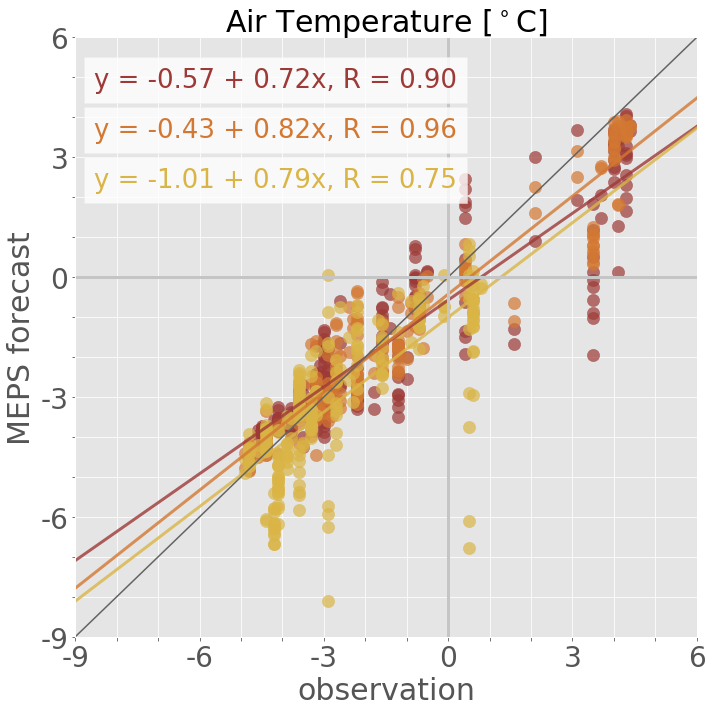
\includegraphics[trim={0.cm 0cm 12.5cm 0cm},clip,
    width=\textwidth]{./fig_sfc_temp/obs_model_20161224_26_00}
     	\caption{}\label{fig:scat:temp2426}
     \end{subfigure}
     
     % label
     \begin{subfigure}[b]{0.49\textwidth}
     	\centering
     	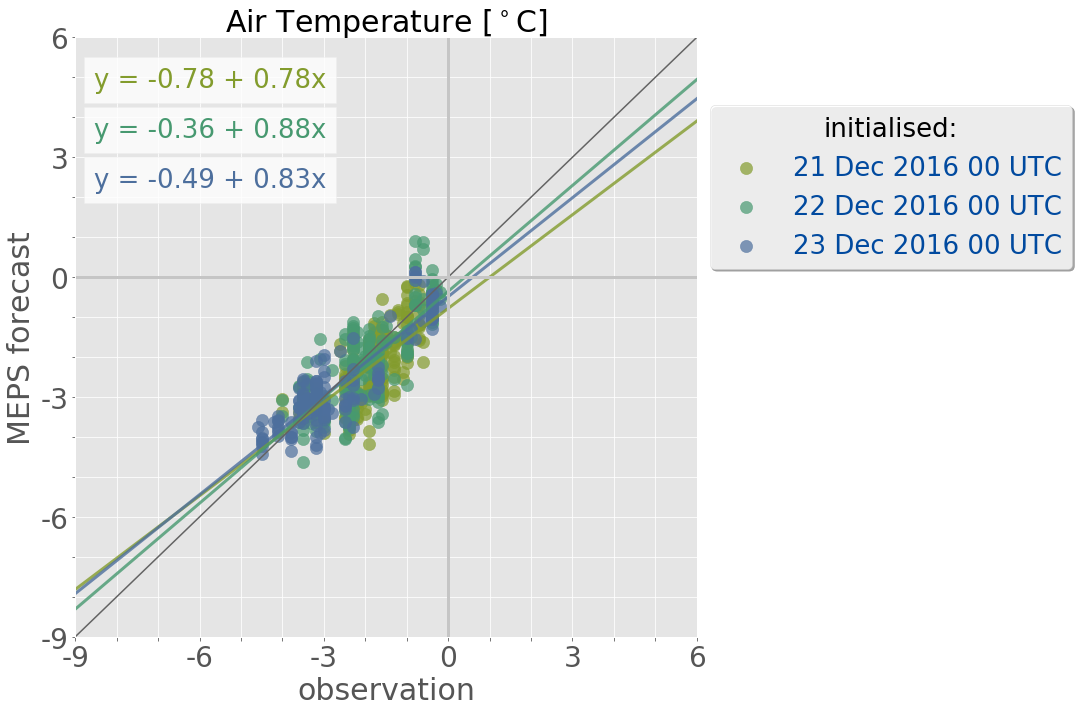
\includegraphics[trim={25.cm 15.5cm 0cm 3.6cm},clip,
    width=0.8\textwidth]{./fig_sfc_temp/obs_model_20161221_23_00}
     \end{subfigure}
     \begin{subfigure}[b]{0.49\textwidth}
     	\centering
     	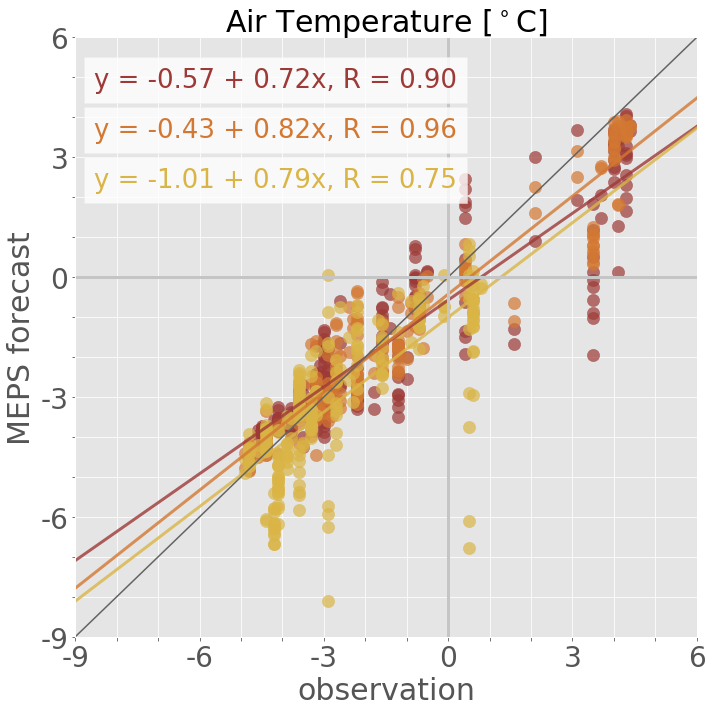
\includegraphics[trim={25.cm 15.5cm 0cm 3.6cm},clip,
    width=0.8\textwidth]{./fig_sfc_temp/obs_model_20161224_26_00}
     \end{subfigure}
\end{figure}
\begin{figure}\ContinuedFloat
     % sfc wd
	\begin{subfigure}[b]{0.49\textwidth}
     	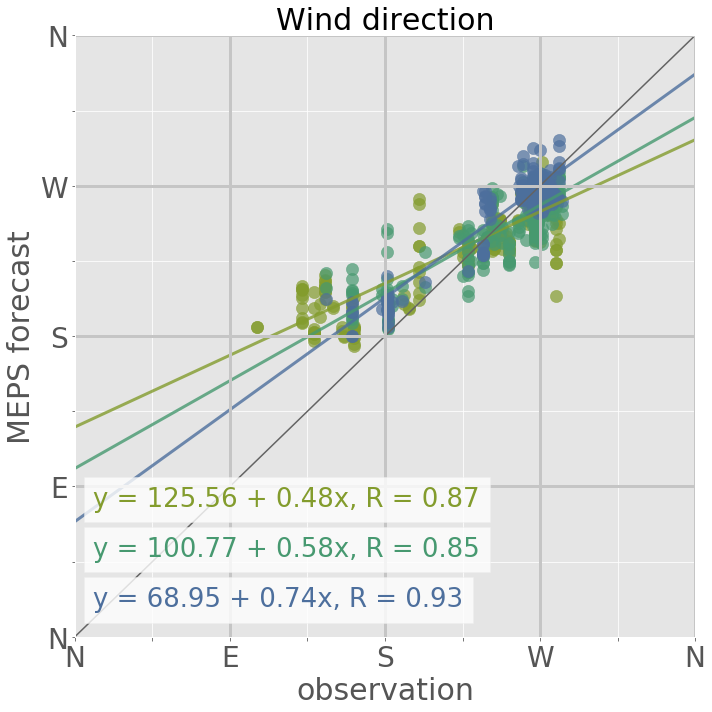
\includegraphics[trim={0.cm 0cm 12.5cm 0cm},clip,
    width=\textwidth]{./fig_sfc_wd/obs_model_20161221_23_00}
     	\caption{}\label{fig:scat:wd2123}
     \end{subfigure}
     %
	\begin{subfigure}[b]{0.49\textwidth}
     	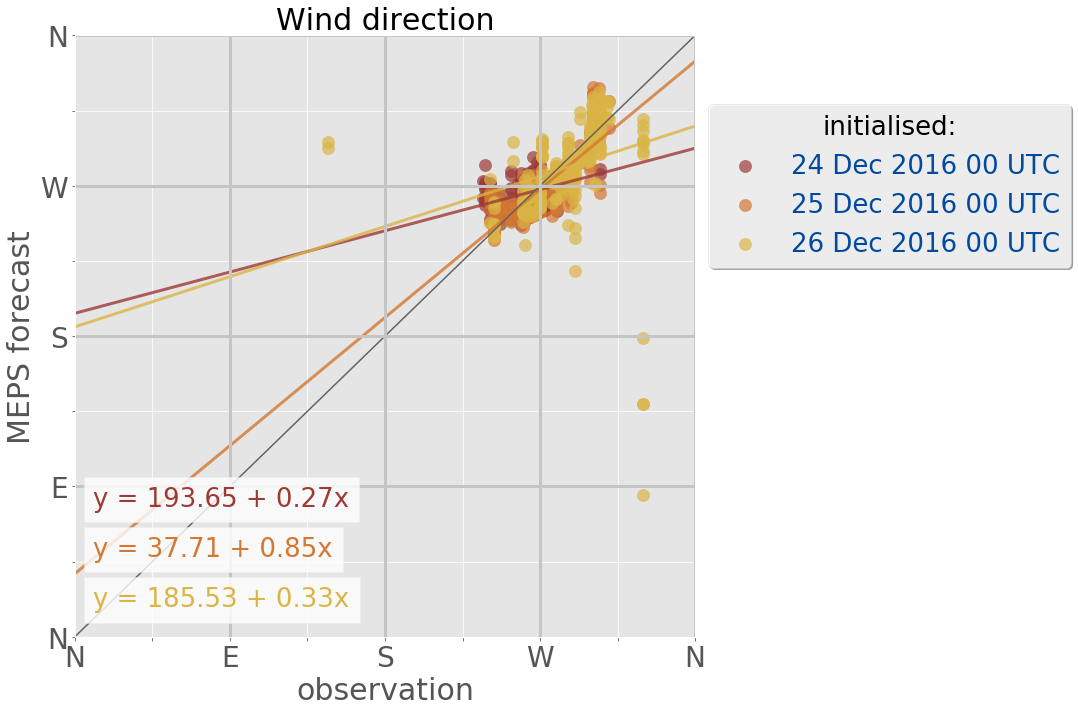
\includegraphics[trim={0.cm 0cm 12.5cm 0cm},clip,
    width=\textwidth]{./fig_sfc_wd/obs_model_20161224_26_00}
     	\caption{}\label{fig:scat:wd2426}
     \end{subfigure}
     % sfc ws
	\begin{subfigure}[b]{0.49\textwidth}
     	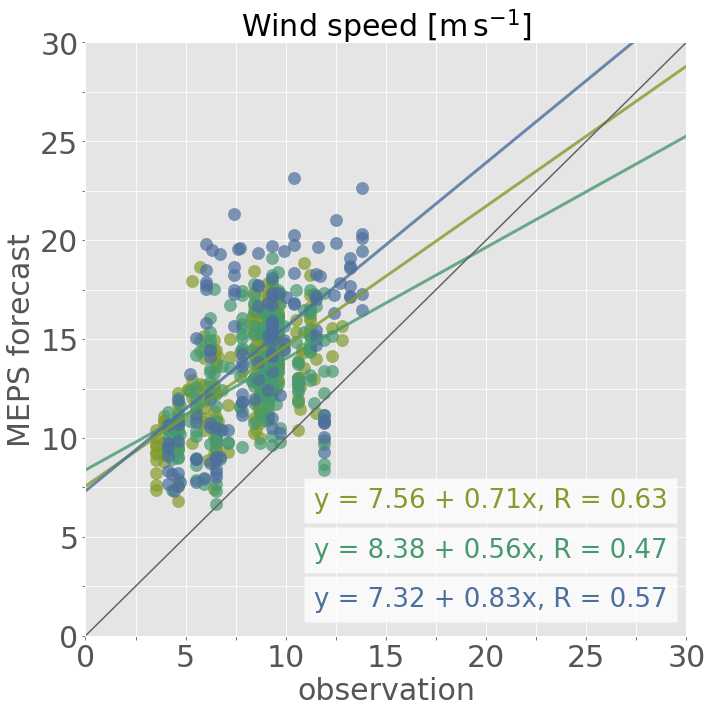
\includegraphics[trim={0.cm 0cm 12.5cm 0cm},clip,
    width=\textwidth]{./fig_sfc_ws/obs_model_20161221_23_00}
     	\caption{}\label{fig:scat:ws2123}
     \end{subfigure}
     %
	\begin{subfigure}[b]{0.49\textwidth}
     	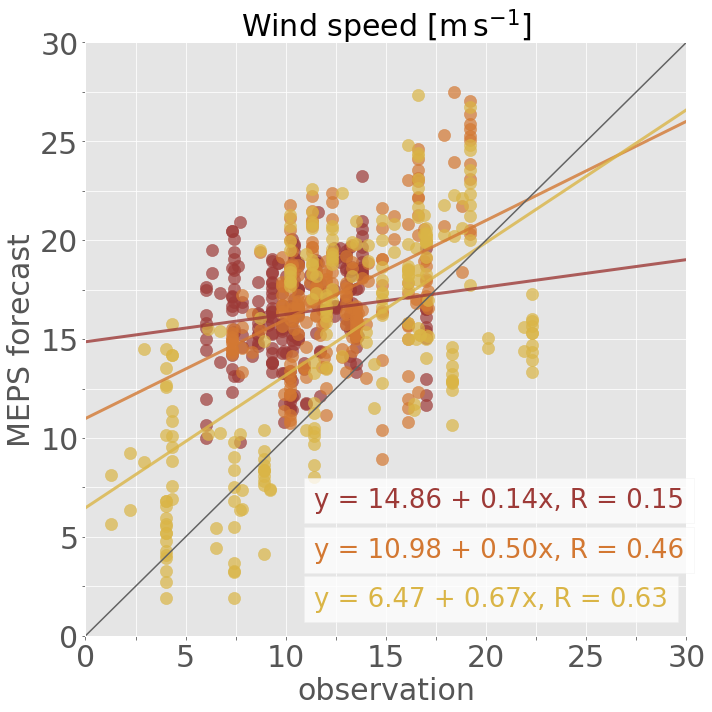
\includegraphics[trim={0.cm 0cm 12.5cm 0cm},clip,
    width=\textwidth]{./fig_sfc_ws/obs_model_20161224_26_00}
     	\caption{}\label{fig:scat:ws2426}
     \end{subfigure}
     % label
     \begin{subfigure}[b]{0.49\textwidth}
     	\centering
     	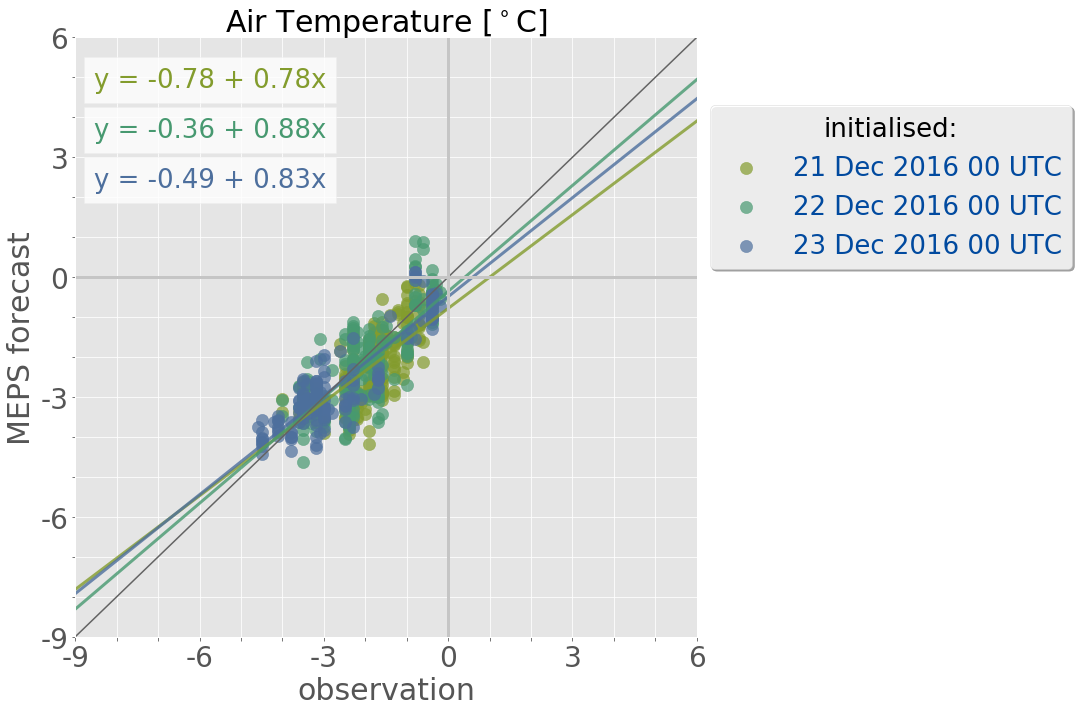
\includegraphics[trim={25.cm 15.5cm 0cm 3.6cm},clip,
    width=0.8\textwidth]{./fig_sfc_temp/obs_model_20161221_23_00}
     \end{subfigure}
     \begin{subfigure}[b]{0.49\textwidth}
     	\centering
     	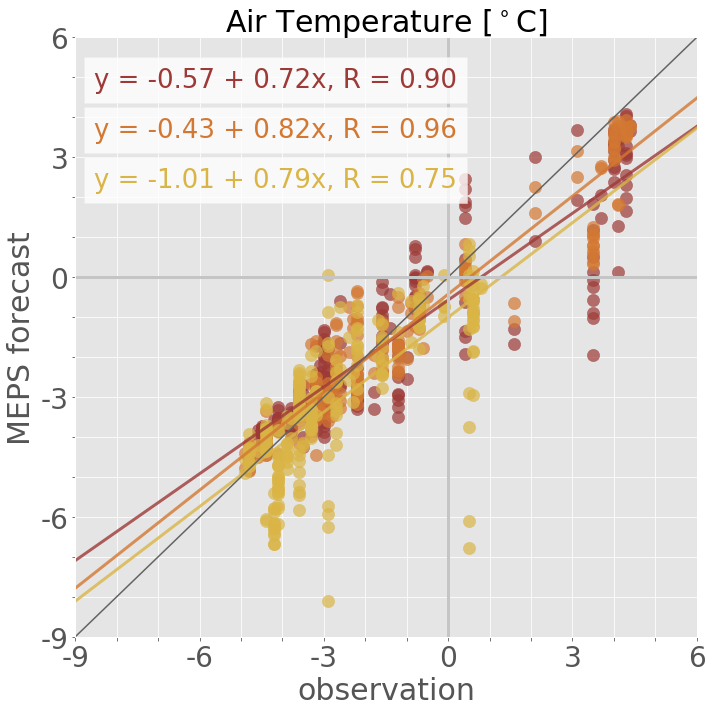
\includegraphics[trim={25.cm 15.5cm 0cm 3.6cm},clip,
    width=0.8\textwidth]{./fig_sfc_temp/obs_model_20161224_26_00}
    \end{subfigure}
\end{figure}
\begin{figure}\ContinuedFloat
     % sfc precip
	\begin{subfigure}[b]{0.49\textwidth}
     	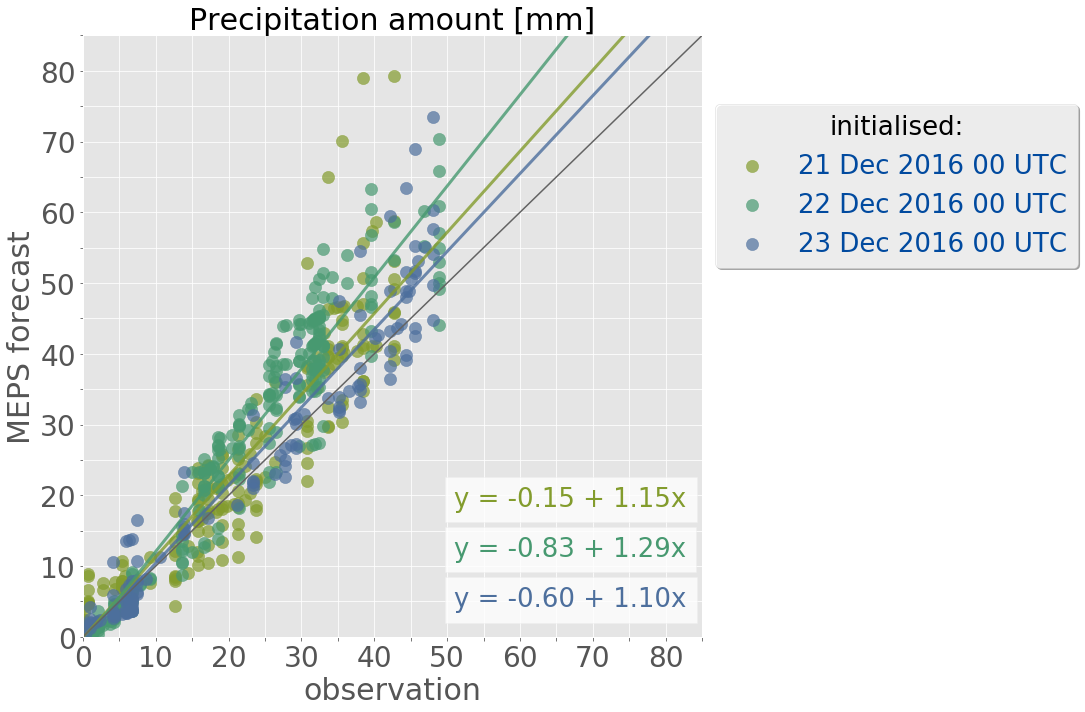
\includegraphics[trim={0.cm 0cm 12.5cm 0cm},clip,
    width=\textwidth]{./fig_sfc_precip/obs_model_20161221_23_00}
     	\caption{}\label{fig:scat:precip2123}
     \end{subfigure}
     %
	\begin{subfigure}[b]{0.49\textwidth}
     	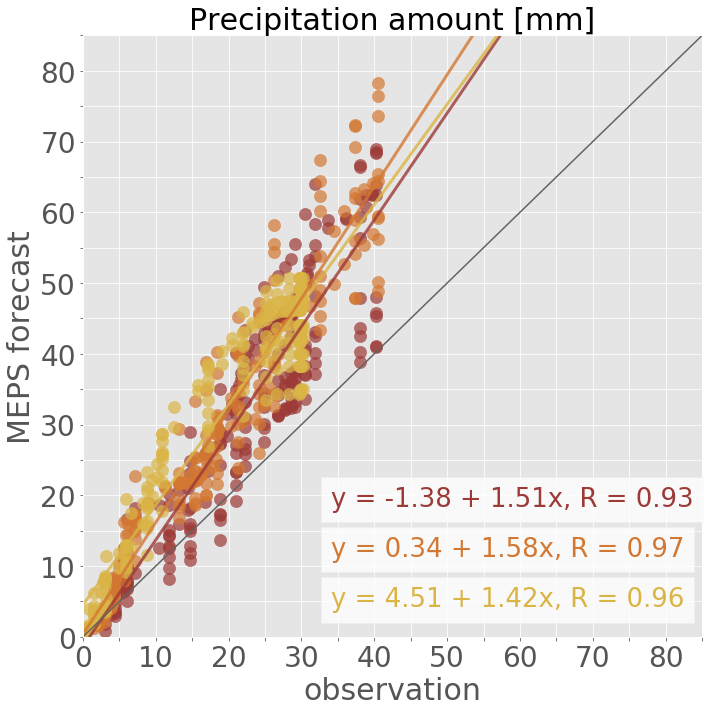
\includegraphics[trim={0.cm 0cm 12.5cm 0cm},clip,
    width=\textwidth]{./fig_sfc_precip/obs_model_20161224_26_00}
     	\caption{}\label{fig:scat:precip2426}
     \end{subfigure}
     % label
     \begin{subfigure}[b]{0.49\textwidth}
     	\centering
     	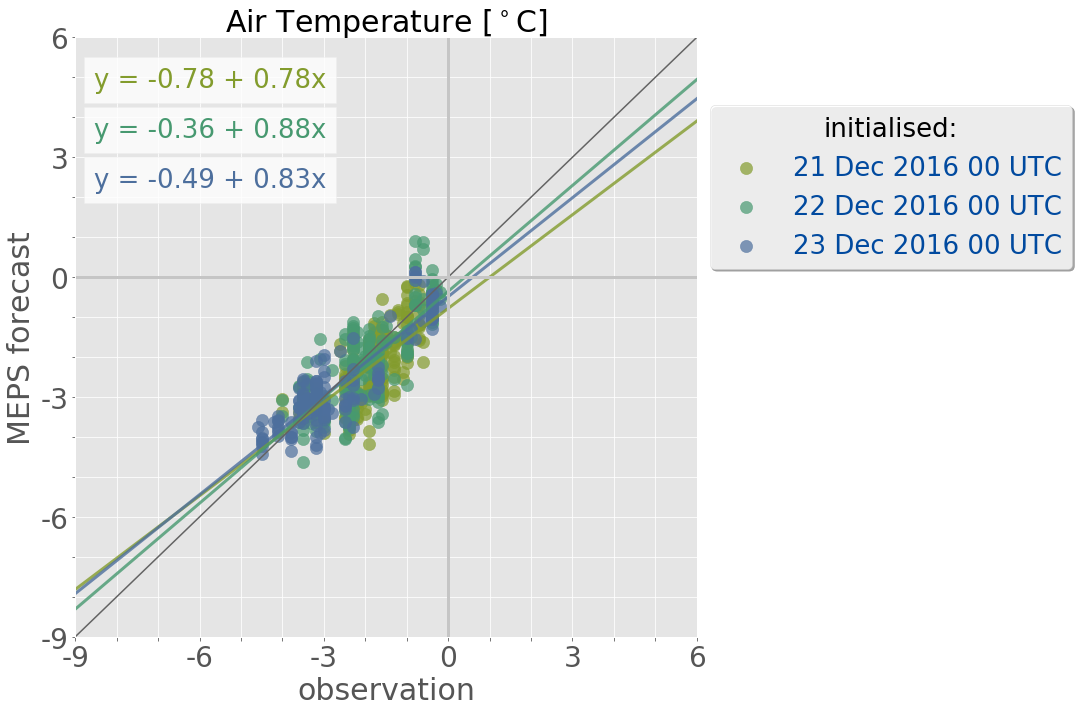
\includegraphics[trim={25.cm 15.5cm 0cm 3.6cm},clip,
    width=0.8\textwidth]{./fig_sfc_temp/obs_model_20161221_23_00}
     \end{subfigure}
     \begin{subfigure}[b]{0.49\textwidth}
     	\centering
     	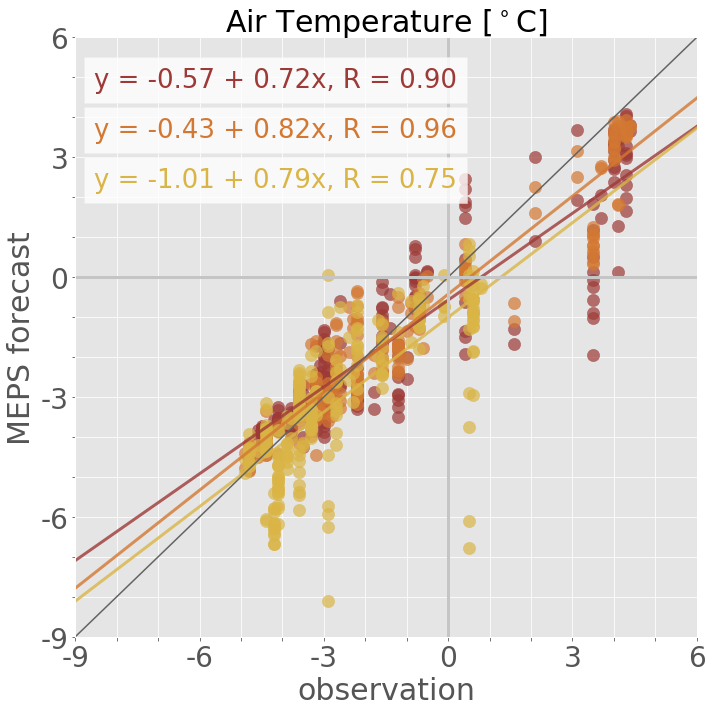
\includegraphics[trim={25.cm 15.5cm 0cm 3.6cm},clip,
    width=0.8\textwidth]{./fig_sfc_temp/obs_model_20161224_26_00}
     \end{subfigure}
     \caption{\SI{48}{\hour} scatter plots for surface observations and ensemble forecasts initialised for \SIrange{21}{23}{\dec} (left column, \protect\subref{fig:scat:pres2123}, \protect\subref{fig:scat:temp2123}, \protect\subref{fig:scat:wd2123}, \protect\subref{fig:scat:ws2123}, \protect\subref{fig:scat:precip2123}) and  for \SIrange{24}{26}{\dec} (right column, \protect\subref{fig:scat:pres2426}, \protect\subref{fig:scat:temp2426}, \protect\subref{fig:scat:wd2426}, \protect\subref{fig:scat:ws2426}, \protect\subref{fig:scat:precip2426}). Upper panel sea level pressure, second \SI{2}{\metre} air temperature, third and forth \SI{10}{\metre} wind direction and speed, respectively, and lowest panel precipitation amount.}\label{fig:scat:obs_meps}
\end{figure}
%%%%%%%%%%%%%%%%%%%%%%%%%%%%%%%%%%%%%%%%%%%%%%
\\
The comparison between the ECMWF analysis shows, that the ensemble member forecast system MEPS covers the prediction of large scale phenomena like frontal boundaries and liquid precipitation at the surface. \Cref{fig:scat:obs_meps} shows the correlation between the observations and the \SI{48}{\hour} forecast. Each variable presents the regression line  for each day and all ensemble members compared to the observations at Haukeliseter.
\\
Sea level pressure has the best correlation under all variables. The best agreement shows on \SI{26}{\dec} when the Christmas storm made landfall and dissipates after the passage of the occluded front at \SI{16}{\UTC}. \cite{dahlgren_comparison_2013} showed that by mixing in large scale information from the boundary condition (ECMWF) into the regional model, the forecast for sea level pressure will be improved. The comparison with observational data showed a declination of forecasts after \SI{24}{\hour}. 
Since the pressure values are in good agreement with the observations are assumed that on \SI{25}{\dec} the warm front did not pass through at Haukeliseter. 
\\
The warm sector passing through on \SI{25}{\dec} was predicted by MEPS and observed at the station. Comparing \Cref{fig:scat:temp2426} shows a moderate correlation between observation and \SI{48}{\hour} forecast. MEPS underestimated the observed temperature, but it estimated it at the correct time. In \cite{muller_arome-metcoop:_2017} it states that after winter 2012 was the temperature bias negative. \Cref{fig:bias:temp} shows for \SIlist{23;26}{\dec} positive as well as negative biases for the individual members. The \SI{25}{\dec}, where the warm sector was observed shows a negative bias, underestimating the temperature when compared to the observation. The mean error for the Norwegian model domain of AROME-MetCoOP estimated by \cite{muller_arome-metcoop:_2017} is smaller than \SI{1.8}{\kelvin} for the surface temperature in December 2014. The forecasts for \SIlist{23;25;26}{\dec} show mean absolute error values of up to \SIlist{0.61;0.77;1.44}{\kelvin}. This shows a good predictability for temperatures of the event. 
\\
According to \cite{muller_arome-metcoop:_2017} are large wind speeds significantly better simulated for AROME-MetCoOp compared to ECMWF's forecast. The wind speeds between \SIrange{3}{13}{\mPs} agreed with observed and forecasted values for the 2014/2015 season where for higher values the accuracy decreased. Mean absolute errors were below \SI{2}{\mPs} for December 2014. 
\\
\Cref{fig:scat:ws2123} and \subref{fig:scat:ws2426} show indeed higher values than the observations at Haukeliseter. The mean absolute error for the Christmas storm is higher at all days. From the three days with frontal passages the \SI{23}{\dec} shows the highest mean absolute error of \SI{6.5}{\mPs}, more than three times as high as the monthly averaged value from \cite{muller_arome-metcoop:_2017}. Their study case in February 2015 showed a large difference between AROME-MetCoOp and ECMWF. While the wind direction of MEPS has a good agreement shows the wind speed larger values over all days. Although MEPS includes ten perturbed ensemble members the insufficiency of AROME-MetCoOp too high wind prediction in extreme situations is not resolved. The regional model wind prediction is still dependent on the intensity of the storm. As \cite{muller_arome-metcoop:_2017} also mentioned are higher wind speeds in general better forecasted in AROME-MetCoOp than in ECMWF. 
\\
Haukeliseter is a measurement site exposed to high wind speeds \citep{wolff_measurements_2013,wolff_derivation_2015} it shows in the results, the positive impact of a high resolution forecast model since it is able to estimate larger scale features. In general were surface parameters well forecasted, only wind wind speed and precipitation accumulation showed overestimation in MEPS. Wind speeds forecasted higher than observations, is probably related to the weakness of wind speed prediction already known from the previous operational model AROME-MetCoOp. On the \SIlist{25;26}{\dec} MEPS also overestimated the precipitation amount at the surface. This will be further discussed in \Cref{sec:sfc_acc}.
%%%%%%%%%%%%%%%%%%%%%%%%%%%%%%%%%%%%%%%%%%%%%%%%%%%%%%%%%%%%%%%%%%%%%%%%%%

%%%%%%%%%%%%%%%%%%%%%%%%%%%%%%%%%%%%%%%%%%%%%%%%%%%%%%%%%%%%%%%%%%%%%%%%%%
%%%%%%%%% Local affects %%%%%%%%%%%%%%
\section{Orographic influence on precipitation}
%%%%%%%%%%%%%%%%%%%%%%%%%%%%%%%%%%%%%%%%%%%%%%%%%%%%%%%%%%%%%%%%%%%%%%%%%%

%%%%%%%%%%%%%%%%%%%%%%%%%%%%%%%%%%%%%%%%%%%%%%%%%%%%%%%%%%%%%%%%%%%%%%%%%
%%%%%%%% Relationship between wind and surface accumulation %%%%%%%%%%%%%%
\section{Relation between surface precipitation amount and wind}\label{sec:sfc_acc}
%%%%%%%%%%%%%%%%%%%%%%%%%%%%%%%%%%%%%%%%%%%%%%%%%%%%%%%%%%%%%%%%%%%%%%%%%





